\documentclass[12pt,a4paper,reqno]{amsart}
\usepackage[T1]{fontenc}
\usepackage[utf8]{inputenc}
\usepackage{lmodern,amsmath,amssymb,amsthm,microtype,enumitem,tasks,tikz,hyperref,needspace}
\newcommand{\krastineszymek}[1]{\tikz[baseline=(current bounding box.center)]{\foreach \x in {#1}{\draw (\x pt,-2.5pt)--(\x pt,2.5pt);}}}
\settasks{label-align=left,label-width=1.5em,label-offset=0.4em,item-indent=1.9em}
\emergencystretch=4em
\setlength{\parindent}{0pt}\setlength{\parskip}{0.6\baselineskip}
\makeatletter
\def\section{\@startsection{section}{1}{\z@}{-1.5\baselineskip plus -.3\baselineskip minus -.2\baselineskip}{0.6\baselineskip}{\normalfont\large\bfseries\raggedright}}
\makeatother
\theoremstyle{plain}\newtheorem{theorem}{Teorema}[section]
\newtheorem{lemma}[theorem]{Lema}\newtheorem{property}[theorem]{Savybė}\newtheorem{proposition}[theorem]{Teiginys}\newtheorem{corollary}[theorem]{Išvada}\newtheorem{conjecture}[theorem]{Hipotezė}
\theoremstyle{definition}
\newtheorem{definition}[theorem]{Apibrėžimas}\newtheorem{fact}[theorem]{Faktas}\newtheorem{example}[theorem]{Pavyzdys}\newtheorem{algorithm}[theorem]{Algoritmas}\newtheorem{question}[theorem]{Klausimas}\newtheorem{exercise}[theorem]{Pratimas}\newtheorem{problem}[theorem]{Uždavinys}\newtheorem{anchorproblem}[theorem]{Atraminis uždavinys}
\theoremstyle{remark}\newtheorem{remark}[theorem]{Pastaba}\newtheorem*{remark*}{Pastaba}
\theoremstyle{definition}\newtheorem*{problem*}{Uždavinys}
\newenvironment{starproblem}{\begingroup\let\numberwithoutstar\thetheorem\renewcommand{\thetheorem}{\numberwithoutstar\textsuperscript{*}}\begin{problem}}{\end{problem}\endgroup}
\newenvironment{staranchorproblem}{\begingroup\let\numberwithoutstar\thetheorem\renewcommand{\thetheorem}{\numberwithoutstar\textsuperscript{*}}\begin{anchorproblem}}{\end{anchorproblem}\endgroup}
\renewcommand{\proofname}{Įrodymas}\newenvironment{solution}[1][]{\par\medskip\Needspace{3\baselineskip}\noindent\textbf{#1.}\par\nobreak\noindent}{\par\medskip}
\newenvironment{answer}{\par\medskip\noindent\textit{Atsakymas.}\enspace}{\par\medskip}\newcommand{\ats}[1]{\par\noindent\textit{Atsakymas.} #1}
\newcommand{\kelias}[1]{\par\smallskip\noindent\textit{#1}\enspace}
\title[Trikampių lygumas]{Trikampių lygumas ir jo taikymai}
\newcommand{\poteme}{Antrasis temos karkaso variantas}
\author{Andrius Berniukevičius}\newcommand{\mokykla}{Vilniaus licėjus}
\makeatletter
\def\@settitle{\begin{center}{\large\bfseries \@title\par}\vspace{0.5em}{\normalsize\bfseries \poteme\par}\end{center}}
\def\@setauthors{\begin{center}\authors\par\vspace{0.3em}\mokykla\par\end{center}}
\makeatother\date{}
\begin{document}\maketitle
\section*{Įvadas}
Kaip iš kelių žinomų atkarpų ar kampų lygybių gauti naujų? Šiame lape mokysimės pasirinkti ir palyginti trikampius, o gautas išvadas taikysime kitiems uždaviniams.

Jau žinome du trikampių lygumo požymius: pagal dvi kraštines ir kampą tarp jų; pagal kraštinę ir du kampus prie jos. Taip pat žinome gretutinių ir kryžminių kampų savybes ir trikampio nelygybę: trikampis su kraštinėmis $a$, $b$, $c$ egzistuoja tada ir tik tada, kai kiekviena kraštinė mažesnė už kitų dviejų sumą. Remsimės ir įprastomis elementariosios geometrijos konstrukcijomis: atkarpos vidurio tašku, kampo pusiaukampine, kampo ir atkarpos atidėjimu (į nurodytą tiesės pusę tai galima padaryti vieninteliu būdu), taip pat tuo, kad per tašką galima nubrėžti vieną duotai tiesei statmeną tiesę. Šios konstrukcijos čia laikomos pradinėmis žiniomis. Paskutinįjį faktą tuo atveju, kai taškas nepriklauso tiesei, vėliau įrodysime (\ref{atr:statmuo} uždavinys).

Naudosimės ir akivaizdžiais taškų išsidėstymo faktais. Dvi skirtingos tiesės turi ne daugiau kaip vieną bendrą tašką. Jei taškas $B$ yra atkarpoje $AC$, tai $AC=AB+BC$. Atkarpa, jungianti taškus, esančius skirtingose tiesės pusėse, tą tiesę kerta. Sakome, kad spindulys $CD$ eina kampo $BCE$ viduje, jei taškas $D$ yra toje pačioje tiesės $CE$ pusėje kaip $B$ ir toje pačioje tiesės $CB$ pusėje kaip $E$. Tada $\angle BCE=\angle BCD+\angle DCE$, todėl kiekvienas iš kampų $BCD$ ir $DCE$ mažesnis už kampą $BCE$, o spindulys $CD$ kerta atkarpą $BE$.

Trikampio kampų sumos šiame dokumente nenaudojame. Žvaigždutė prie uždavinio numerio žymi sunkesnį uždavinį. Kai brėžinio nėra, nubraižykite jį patys.
\section{Lygumo įrodymo užrašymas}
Lygių trikampių atitinkamos kraštinės ir kampai lygūs. Užraše $\triangle ABC=\triangle DEF$ atitinka tose pačiose vietose esančios viršūnės: $A$ ir $D$, $B$ ir $E$, $C$ ir $F$. Šiame skyriuje lygius trikampius dar rasime brėžinyje; vėliau juos teks susikurti patiems.
\begin{problem}\label{uzd:breziniai-lygumas-01}
Kiekviename brėžinyje vienodais brūkšneliais pažymėtos atkarpos yra lygios, o vienodais lankeliais pažymėti kampai yra lygūs. Pažymėtas atkarpų susikirtimo taškas priklauso abiem atkarpoms. Remdamiesi šiais duomenimis, raskite po du lygius trikampius ir pagrįskite jų lygumą. Atkreipkite dėmesį į bendrus elementus ir kryžminius kampus: jie atskirai nepažymėti kaip lygūs, todėl paaiškinkite, kodėl jie lygūs. Naudokite tik du jau žinomus lygumo požymius. Pirmasis punktas – pavyzdys. Atitinkamas viršūnes užrašykite ta pačia tvarka.
\end{problem}
\par\medskip\Needspace{15\baselineskip}
\noindent\textbf{(1)}
\begin{center}
\begin{tikzpicture}[scale=0.9,baseline=(current bounding box.center)]
\coordinate (A) at (-1.85000,0.00000);
\coordinate (O) at (0.00000,0.00000);
\coordinate (C) at (1.85000,0.00000);
\coordinate (B) at (-0.80000,1.45000);
\coordinate (D) at (0.80000,-1.45000);
\draw (A)--(C);
\draw (B)--(D);
\draw (A)--(B);
\draw (C)--(D);
\node at ([shift={(-0.250cm,0.000cm)}]A) {$A$};
\node at ([shift={(0.250cm,0.000cm)}]C) {$C$};
\node at ([shift={(-0.080cm,0.240cm)}]B) {$B$};
\node at ([shift={(0.080cm,-0.240cm)}]D) {$D$};
\node at ([shift={(-0.180cm,-0.200cm)}]O) {$O$};
\path (A)--(O) node[midway,sloped,inner sep=0pt] {\krastineszymek{0}}
      (O)--(C) node[midway,sloped,inner sep=0pt] {\krastineszymek{0}};
\draw (-1.7034,0.2025) arc[start angle=54.0903,end angle=-0.0000,radius=0.250];
\draw (1.7034,-0.2025) arc[start angle=-125.9097,end angle=-180.0000,radius=0.250];
\end{tikzpicture}
\end{center}
Palyginkime trikampius $AOB$ ir $COD$:
\begin{itemize}[nosep]
\item $AO=CO$ (duota, pažymėta vienu brūkšneliu);
\item $\angle BAO=\angle DCO$ (duota, pažymėta vienu lankeliu);
\item $\angle AOB=\angle COD$ (kryžminiai kampai).
\end{itemize}
Lygūs kampai yra prie atitinkamai lygių kraštinių $AO$ ir $CO$. Todėl $\triangle AOB=\triangle COD$ pagal kraštinę ir du kampus prie jos.

\par\medskip\Needspace{15\baselineskip}
\noindent\textbf{(2)}
\begin{center}
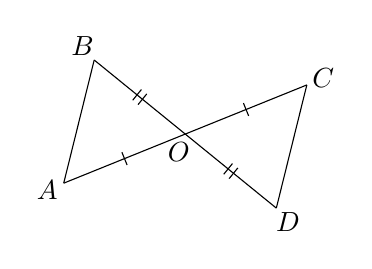
\begin{tikzpicture}[scale=0.9,baseline=(current bounding box.center)]
\coordinate (A) at (-1.71529,-0.69302);
\coordinate (O) at (0.00000,0.00000);
\coordinate (C) at (1.71529,0.69302);
\coordinate (B) at (-1.28493,1.04473);
\coordinate (D) at (1.28493,-1.04473);
\draw (A)--(C);
\draw (B)--(D);
\draw (A)--(B);
\draw (C)--(D);
\node at ([shift={(-0.232cm,-0.094cm)}]A) {$A$};
\node at ([shift={(0.232cm,0.094cm)}]C) {$C$};
\node at ([shift={(-0.164cm,0.193cm)}]B) {$B$};
\node at ([shift={(0.164cm,-0.193cm)}]D) {$D$};
\node at ([shift={(-0.092cm,-0.253cm)}]O) {$O$};
\path (A)--(O) node[midway,sloped,inner sep=0pt] {\krastineszymek{0}}
      (O)--(C) node[midway,sloped,inner sep=0pt] {\krastineszymek{0}}
      (B)--(O) node[midway,sloped,inner sep=0pt] {\krastineszymek{-1.25,1.25}}
      (O)--(D) node[midway,sloped,inner sep=0pt] {\krastineszymek{-1.25,1.25}};
\end{tikzpicture}
\end{center}
Palyginkime trikampius $\underline{\hspace{1.3cm}}$ ir $\underline{\hspace{1.3cm}}$:\par
\rule{0pt}{1.2em}\dotfill\par
\rule{0pt}{1.2em}\dotfill\par
\rule{0pt}{1.2em}\dotfill\par
Todėl $\triangle\underline{\hspace{1cm}}=\triangle\underline{\hspace{1cm}}$ pagal \dotfill .\par

\par\medskip\Needspace{15\baselineskip}
\noindent\textbf{(3)}
\begin{center}
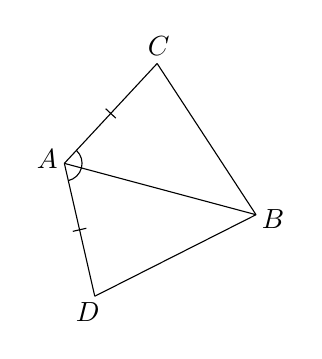
\begin{tikzpicture}[scale=0.9,baseline=(current bounding box.center)]
\coordinate (A) at (0.00000,0.00000);
\coordinate (B) at (2.70459,-0.72469);
\coordinate (C) at (1.30933,1.40914);
\coordinate (D) at (0.42934,-1.87501);
\draw (A)--(B);
\draw (A)--(C);
\draw (B)--(C);
\draw (A)--(D);
\draw (B)--(D);
\node at ([shift={(-0.241cm,0.065cm)}]A) {$A$};
\node at ([shift={(0.241cm,-0.065cm)}]B) {$B$};
\node at ([shift={(0.023cm,0.242cm)}]C) {$C$};
\node at ([shift={(-0.101cm,-0.221cm)}]D) {$D$};
\path (A)--(C) node[midway,sloped,inner sep=0pt] {\krastineszymek{0}}
      (A)--(D) node[midway,sloped,inner sep=0pt] {\krastineszymek{0}};
\draw (0.1702,0.1831) arc[start angle=47.1027,end angle=-15.0000,radius=0.250];
\draw (0.0558,-0.2437) arc[start angle=-77.1027,end angle=-15.0000,radius=0.250];
\end{tikzpicture}
\end{center}
Palyginkime trikampius $\underline{\hspace{1.3cm}}$ ir $\underline{\hspace{1.3cm}}$:\par
\rule{0pt}{1.2em}\dotfill\par
\rule{0pt}{1.2em}\dotfill\par
\rule{0pt}{1.2em}\dotfill\par
Todėl $\triangle\underline{\hspace{1cm}}=\triangle\underline{\hspace{1cm}}$ pagal \dotfill .\par

\par\medskip\Needspace{15\baselineskip}
\noindent\textbf{(4)}
\begin{center}
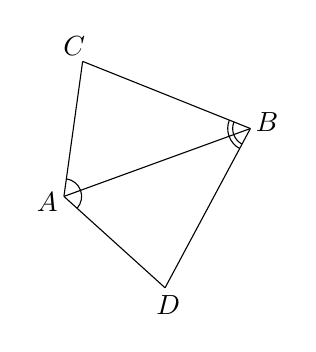
\begin{tikzpicture}[scale=0.9,baseline=(current bounding box.center)]
\coordinate (A) at (0.00000,0.00000);
\coordinate (B) at (2.63114,0.95766);
\coordinate (C) at (0.26429,1.90530);
\coordinate (D) at (1.42716,-1.28966);
\draw (A)--(B);
\draw (A)--(C);
\draw (B)--(C);
\draw (A)--(D);
\draw (B)--(D);
\node at ([shift={(-0.235cm,-0.086cm)}]A) {$A$};
\node at ([shift={(0.235cm,0.086cm)}]B) {$B$};
\node at ([shift={(-0.120cm,0.212cm)}]C) {$C$};
\node at ([shift={(0.044cm,-0.239cm)}]D) {$D$};
\draw (0.0343,0.2476) arc[start angle=82.1027,end angle=20.0000,radius=0.250];
\draw (0.1855,-0.1676) arc[start angle=-42.1027,end angle=20.0000,radius=0.250];
\draw (2.3962,0.8722) arc[start angle=-160.0000,end angle=-201.8202,radius=0.250];
\draw (2.3304,0.8482) arc[start angle=-160.0000,end angle=-201.8202,radius=0.320];
\draw (2.3962,0.8722) arc[start angle=-160.0000,end angle=-118.1798,radius=0.250];
\draw (2.3304,0.8482) arc[start angle=-160.0000,end angle=-118.1798,radius=0.320];
\end{tikzpicture}
\end{center}
Įrodymas:\par
\rule{0pt}{1.2em}\dotfill\par
\rule{0pt}{1.2em}\dotfill\par
\rule{0pt}{1.2em}\dotfill\par
\rule{0pt}{1.2em}\dotfill\par
\rule{0pt}{1.2em}\dotfill\par

\par\medskip\Needspace{15\baselineskip}
\noindent\textbf{(5)}
\begin{center}
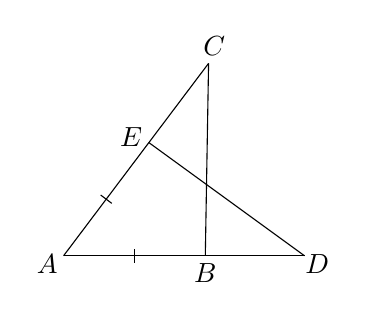
\begin{tikzpicture}[scale=0.9,baseline=(current bounding box.center)]
\coordinate (A) at (0.00000,0.00000);
\coordinate (B) at (2.00000,0.00000);
\coordinate (D) at (3.40000,0.00000);
\coordinate (C) at (2.04617,2.71536);
\coordinate (E) at (1.20363,1.59727);
\draw (A)--(D);
\draw (A)--(C);
\draw (B)--(C);
\draw (D)--(E);
\node at ([shift={(-0.230cm,-0.120cm)}]A) {$A$};
\node at ([shift={(0.000cm,-0.250cm)}]B) {$B$};
\node at ([shift={(0.180cm,-0.120cm)}]D) {$D$};
\node at ([shift={(0.080cm,0.240cm)}]C) {$C$};
\node at ([shift={(-0.250cm,0.080cm)}]E) {$E$};
\path (A)--(B) node[midway,sloped,inner sep=0pt] {\krastineszymek{0}}
      (A)--(E) node[midway,sloped,inner sep=0pt] {\krastineszymek{0}};
\end{tikzpicture}
\end{center}
Duota: $AB=AE$ ir $AC=AD$.

Įrodymas:\par
\rule{0pt}{1.2em}\dotfill\par
\rule{0pt}{1.2em}\dotfill\par
\rule{0pt}{1.2em}\dotfill\par
\rule{0pt}{1.2em}\dotfill\par
\rule{0pt}{1.2em}\dotfill\par


\begin{problem}\label{uzd:lygybe-atitikimas-01} Žinoma, kad $\triangle ABC=\triangle PQR$. Kurios kraštinės atitinka $AB$ ir $AC$? Kurie kampai atitinka $\angle ABC$ ir $\angle BAC$? Užrašykite likusių atitinkamų kraštinių ir kampų lygybes. \end{problem}
\begin{problem}\label{uzd:lygybe-sas-01} Duota $AB=FE$, $AC=FD$, $\angle BAC=\angle EFD$. Įrodykite, kad trikampiai $ABC$ ir $FED$ lygūs. Kuri kraštinė lygi $BC$? \end{problem}
\begin{problem}\label{uzd:lygybe-asa-01} Trikampiuose $ABC$ ir $KLM$ žinoma: $AB=KL$, $\angle BAC=\angle LKM$, $\angle ABC=\angle KLM$. Įrodykite, kad trikampiai lygūs, ir nurodykite $AC$ atitinkančią kraštinę. \end{problem}
\begin{problem}\label{uzd:lygybe-klaida-01} Mokinys tvirtina: „Jeigu $AB=DE$, $AC=DF$ ir $\angle ABC=\angle DEF$, tai trikampiai lygūs pagal dvi kraštines ir kampą tarp jų.“ Paaiškinkite, kodėl nurodytu požymiu taip remtis negalima. Ar užtektų papildomos sąlygos $\angle BAC=\angle EDF$? \end{problem}
\begin{problem}\label{uzd:lygybe-ssa-01} Ar iš dviejų kraštinių ir kampo, kuris nėra tarp jų, lygybės išplaukia trikampių lygumas? Ištirkite tokį pavyzdį. Pasirinkite taškus $A$, $C$, $D$, nesančius vienoje tiesėje, taip, kad $AC=AD$, ir pratęskite atkarpą $CD$ už taško $D$ iki taško $B$. Kurios trikampių $ABC$ ir $ABD$ kraštinės ir kampai lygūs? Ar šie trikampiai lygūs? \end{problem}
\begin{center}
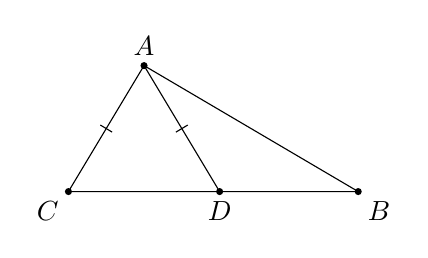
\begin{tikzpicture}[scale=.8]
\coordinate (A) at (1.2,2);\coordinate (C) at (0,0);\coordinate (D) at (2.4,0);\coordinate (B) at (4.6,0);
\draw (C)--(B) (A)--(C) (A)--(D) (A)--(B);
\path (A)--(C) node[midway,sloped,inner sep=0pt] {\krastineszymek{0}}
      (A)--(D) node[midway,sloped,inner sep=0pt] {\krastineszymek{0}};
\foreach \p/\pos in {A/above,C/below left,D/below,B/below right} {\fill (\p) circle (1.6pt) node[\pos] {$\p$};}
\end{tikzpicture}
\end{center}
\begin{problem}\label{uzd:lygybe-susikirtimas-01} Atkarpos $AC$ ir $BD$ kertasi taške $O$. Duota $AO=OC$ ir $BO=OD$. Įrodykite, kad $AB=CD$ ir $AD=CB$. Raskite dar dvi lygių trikampių poras, kurių viršūnė nėra taškas $O$, ir pagrįskite jų lygumą. \end{problem}
\begin{center}
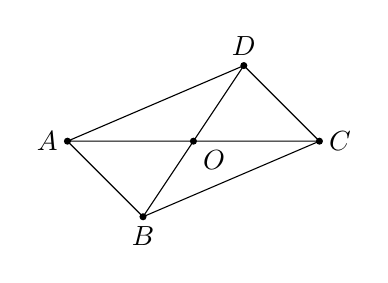
\begin{tikzpicture}[scale=0.8]
\coordinate (O) at (0,0); \coordinate (A) at (-2,0); \coordinate (C) at (2,0); \coordinate (B) at (-.8,-1.2); \coordinate (D) at (.8,1.2);
\draw (A)--(C) (B)--(D) (A)--(B) (C)--(D) (A)--(D) (B)--(C);
\foreach \p/\pos in {A/left,B/below,D/above,C/right,O/below right} {\fill (\p) circle (1.6pt) node[\pos] {$\p$};}
\end{tikzpicture}
\end{center}
\begin{problem}\label{uzd:lygybe-pusiaukampine-01} Taškas $D$ yra trikampio $ABC$ kraštinėje $BC$, $AB=AC$, o $AD$ yra kampo $BAC$ pusiaukampinė. Įrodykite, kad $BD=DC$ ir $AD\perp BC$. \end{problem}
\section{Lygiašonis trikampis}
\kelias{Kur einame.} Iki šiol lygius trikampius radome brėžinyje. Dabar patys nuspręsime, kokią liniją nubrėžti, kad atsirastų du lygūs trikampiai: lygiašoniame trikampyje tokia linija yra pusiaukampinė iš viršūnės. Atkreipkite dėmesį ir į kitą gudrybę: trikampį galima palyginti su juo pačiu, tik viršūnes surašius kita tvarka (\ref{atr:lygias-atvirkstine} uždavinys).
\Needspace{10\baselineskip}
\begin{definition}\label{apib:lygias-trikampis} Trikampis, kurio dvi kraštinės lygios, vadinamas \emph{lygiašoniu}. Šios kraštinės vadinamos šoninėmis, o trečioji – pagrindu.
\begin{center}
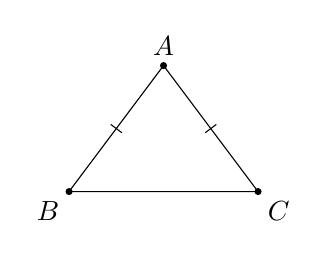
\begin{tikzpicture}[scale=.8]
\coordinate (A) at (1.5,2);\coordinate (B) at (0,0);\coordinate (C) at (3,0);
\draw (A)--(B) node[midway,sloped,inner sep=0pt] {\krastineszymek{0}}--(C)--(A) node[midway,sloped,inner sep=0pt] {\krastineszymek{0}};
\foreach \p/\pos in {A/above,B/below left,C/below right} {\fill (\p) circle (1.6pt) node[\pos] {$\p$};}
\end{tikzpicture}
\end{center}
\end{definition}
\begin{problem}\label{uzd:lygias-supratimas-01} Trikampyje $ABC$ duota $AB=AC$. Nurodykite pagrindą ir kampus prie pagrindo. Ar trikampis, kurio visos kraštinės lygios, atitinka apibrėžimą? Ar galima pasirinkti bet kurią jo kraštinę pagrindu? \end{problem}
\begin{starproblem}\label{uzd:lygias-perimetras-01} Lygiašonio trikampio perimetras yra $20$ cm, o viena kraštinė lygi $6$ cm. Raskite likusių dviejų kraštinių ilgius. \end{starproblem}
\begin{anchorproblem}[Lygiašonio trikampio kampų prie pagrindo savybė]\label{atr:lygias-pagrindo-kampai} Nubrėžkite lygiašonio trikampio kampo tarp šoninių kraštinių pusiaukampinę ir įrodykite, kad kampai prie pagrindo lygūs. \end{anchorproblem}
\begin{problem}\label{uzd:lygias-kampai-01} Trikampyje $ABC$ duota $AB=AC$. Raskite $\angle ACB$, jei $\angle ABC=38^\circ$. Ar iš šių duomenų išplaukia, kad $AB=BC$? \end{problem}
\begin{problem}\label{uzd:lygias-kampai-02} Trikampyje $PQR$ duota $PQ=QR$, $\angle QPR=2x+10^\circ$, $\angle PRQ=3x-5^\circ$. Raskite $x$ ir abu nurodytus kampus. \end{problem}
\begin{anchorproblem}[Lygiašonio trikampio požymis]\label{atr:lygias-atvirkstine} Įrodykite: jei du trikampio kampai lygūs, tai prieš juos esančios kraštinės lygios. \end{anchorproblem}
\begin{problem}\label{uzd:lygias-atvirkstine-01} Trikampyje $ABC$ žinoma, kad $\angle ABC=\angle BCA$ ir $AB=7$ cm. Raskite $AC$. \end{problem}
\begin{problem}\label{uzd:lygias-atvirkstine-02} Trikampyje $KLM$ žinoma, kad $\angle KLM=\angle LKM$. Kurios dvi trikampio kraštinės lygios? Paaiškinkite, kodėl kampai $K$ ir $M$ nebūtinai lygūs. \end{problem}
\begin{anchorproblem}\label{atr:lygias-pusiaukrastine} Trikampyje $ABC$ duota $AB=AC$, o $M$ yra $BC$ vidurio taškas. Įrodykite, kad pusiaukraštinė $AM$ yra ir aukštinė, ir kampo $BAC$ pusiaukampinė. \end{anchorproblem}
\begin{problem}\label{uzd:lygias-pusiaukrastine-01} Trikampyje $ABC$ duota $AB=AC$, $BM=MC$ ir $\angle BAM=27^\circ$. Raskite $\angle MAC$ ir $\angle AMB$. \end{problem}
\begin{problem}\label{uzd:lygias-aukstine-01} Trikampyje $ABC$ duota $AB=AC$, $D$ yra kraštinėje $BC$ ir $AD\perp BC$. Įrodykite, kad $BD=DC$ ir $\angle BAD=\angle DAC$. \end{problem}
\begin{problem}\label{uzd:lygias-pusiaukampines-01} Trikampyje $ABC$ duota $AB=AC$. Kampų $ABC$ ir $ACB$ pusiaukampinės kerta kraštines $AC$ ir $AB$ atitinkamai taškuose $D$ ir $E$. Įrodykite, kad $BD=CE$. \end{problem}
\Needspace{10\baselineskip}
\begin{definition}\label{apib:lygiakrastis} Trikampis, kurio visos trys kraštinės lygios, vadinamas \emph{lygiakraščiu}.
\begin{center}
\begin{tikzpicture}[scale=.8]
\coordinate (A) at (1.5,2.59808);\coordinate (B) at (0,0);\coordinate (C) at (3,0);
\draw (A)--(B) node[midway,sloped,inner sep=0pt] {\krastineszymek{0}}--(C) node[midway,sloped,inner sep=0pt] {\krastineszymek{0}}--(A) node[midway,sloped,inner sep=0pt] {\krastineszymek{0}};
\foreach \p/\pos in {A/above,B/below left,C/below right} {\fill (\p) circle (1.6pt) node[\pos] {$\p$};}
\end{tikzpicture}
\end{center}
\end{definition}
\begin{problem}\label{uzd:lygiakrastis-supratimas-01} Ar kiekvienas lygiakraštis trikampis yra lygiašonis? Ar kiekvienas lygiašonis yra lygiakraštis? Pateikite pavyzdį arba paaiškinkite. \end{problem}
\begin{anchorproblem}[Lygiakraščio trikampio savybė ir požymis]\label{atr:lygiakrastis-kampai} Įrodykite: lygiakraščio trikampio visi kampai lygūs; jei visi trikampio kampai lygūs, tai trikampis lygiakraštis. \end{anchorproblem}
\begin{problem}\label{uzd:lygiakrastis-kampai-01} Trikampyje $ABC$ duota $AB=BC=CA$. Palyginkite $\angle BAC$ ir $\angle BCA$. Ar iš čia galima teigti, kad abu šie kampai yra po $60^\circ$, nepasitelkus papildomo fakto? \end{problem}
\section{Trečiasis trikampių lygumo požymis}
\kelias{Kur einame.} Abiem žinomiems požymiams reikėjo kampų. Ar trikampį nusako vien jo kraštinės? Įrodymo idėja tokia: du trikampius sustatome taip, kad susidarytų du lygiašoniai trikampiai su bendru pagrindu, ir pasiremiame jų kampais prie pagrindo. Šį derinį vėl sutiksime vidurio statmens skyriuje. Įrodyme teks nagrinėti kelis taškų išsidėstymo atvejus: brėžinys rodo tik vieną iš jų.
\begin{staranchorproblem}[Trikampių lygumo požymis pagal tris kraštines]\label{atr:sss-poz}

Duoti trikampiai $ABC$ ir $DEF$, kurių $AB=DF$, $BC=FE$ ir $AC=DE$. Lygios kraštinės pažymėtos vienodu brūkšnelių skaičiumi. Įrodysime, kad šie trikampiai lygūs.
\begin{center}
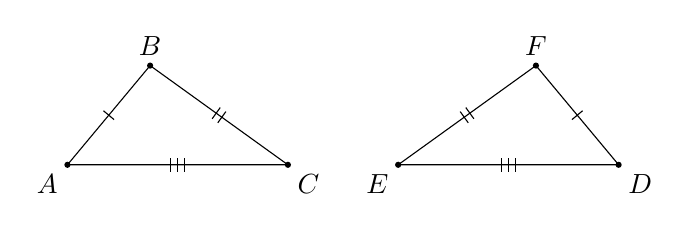
\begin{tikzpicture}[scale=.7]
\coordinate (A) at (0,0);\coordinate (B) at (1.5,1.8);\coordinate (C) at (4,0);
\coordinate (D) at (10,0);\coordinate (F) at (8.5,1.8);\coordinate (E) at (6,0);
\draw (A)--(B) node[midway,sloped,inner sep=0pt] {\krastineszymek{0}}--(C) node[midway,sloped,inner sep=0pt] {\krastineszymek{-1.25,1.25}}--(A) node[midway,sloped,inner sep=0pt] {\krastineszymek{-2.5,0,2.5}};
\draw (D)--(F) node[midway,sloped,inner sep=0pt] {\krastineszymek{0}}--(E) node[midway,sloped,inner sep=0pt] {\krastineszymek{-1.25,1.25}}--(D) node[midway,sloped,inner sep=0pt] {\krastineszymek{-2.5,0,2.5}};
\foreach \p/\pos in {A/below left,B/above,C/below right,D/below right,F/above,E/below left}
{\fill (\p) circle (1.6pt) node[\pos] {$\p$};}
\end{tikzpicture}
\end{center}
\begin{enumerate}[label=\alph*),leftmargin=*]
\item Kitoje tiesės $AC$ pusėje nei taškas $B$ atidėkite kampą $CAK$, lygų kampui $EDF$, o jo kraštinėje – atkarpą $AK=DF$. Nubrėžkite atkarpas $KC$ ir $BK$. Įrodykite, kad $\triangle AKC=\triangle DFE$, ir iš čia išveskite, kad $AK=AB$ ir $CK=CB$.
\begin{center}
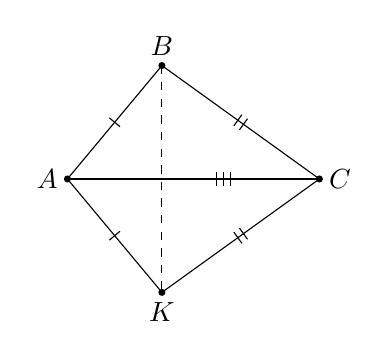
\begin{tikzpicture}[scale=.8]
\coordinate (A) at (0,0);\coordinate (B) at (1.5,1.8);\coordinate (C) at (4,0);\coordinate (K) at (1.5,-1.8);
\draw (A)--(B) node[midway,sloped,inner sep=0pt] {\krastineszymek{0}}--(C) node[midway,sloped,inner sep=0pt] {\krastineszymek{-1.25,1.25}}--(K) node[midway,sloped,inner sep=0pt] {\krastineszymek{-1.25,1.25}}--(A) node[midway,sloped,inner sep=0pt] {\krastineszymek{0}};
\draw (A)--(C) node[pos=.62,sloped,inner sep=0pt] {\krastineszymek{-2.5,0,2.5}};
\draw[dashed] (B)--(K);
\foreach \p/\pos in {A/left,B/above,C/right,K/below}
{\fill (\p) circle (1.6pt) node[\pos] {$\p$};}
\end{tikzpicture}
\end{center}
\item Taškai $B$ ir $K$ yra skirtingose tiesės $AC$ pusėse, todėl atkarpa $BK$ kerta šią tiesę; sankirtos tašką pažymėkite $X$. Įrodykite, kad $\angle ABC=\angle AKC$, atskirai išnagrinėdami tris atvejus: $X$ yra tarp $A$ ir $C$; $X$ sutampa su $A$ arba su $C$; $X$ yra už atkarpos $AC$.
\begin{center}
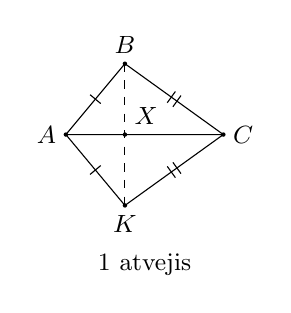
\begin{tikzpicture}[scale=.5,font=\small]
\coordinate (A) at (0,0);\coordinate (C) at (4,0);\coordinate (B) at (1.5,1.8);\coordinate (K) at (1.5,-1.8);\coordinate (X) at (1.5,0);
\draw (A)--(B)--(C)--(K)--cycle (A)--(C);
\draw[dashed] (B)--(K);
\path (A)--(B) node[midway,sloped,inner sep=0pt] {\krastineszymek{0}}
      (A)--(K) node[midway,sloped,inner sep=0pt] {\krastineszymek{0}}
      (B)--(C) node[midway,sloped,inner sep=0pt] {\krastineszymek{-1.25,1.25}}
      (K)--(C) node[midway,sloped,inner sep=0pt] {\krastineszymek{-1.25,1.25}};
\foreach \p/\pos in {A/left,B/above,C/right,K/below,X/above right} {\fill (\p) circle (1.6pt) node[\pos] {$\p$};}
\node at (2,-3.3) {1 atvejis};
\end{tikzpicture}\hspace{1.2em}
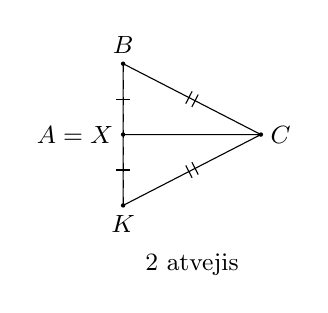
\begin{tikzpicture}[scale=.5,font=\small]
\coordinate (A) at (0,0);\coordinate (C) at (3.5,0);\coordinate (B) at (0,1.8);\coordinate (K) at (0,-1.8);
\draw (A)--(B)--(C)--(K)--cycle (A)--(C);
\draw[dashed] (B)--(K);
\path (A)--(B) node[midway,sloped,inner sep=0pt] {\krastineszymek{0}}
      (A)--(K) node[midway,sloped,inner sep=0pt] {\krastineszymek{0}}
      (B)--(C) node[midway,sloped,inner sep=0pt] {\krastineszymek{-1.25,1.25}}
      (K)--(C) node[midway,sloped,inner sep=0pt] {\krastineszymek{-1.25,1.25}};
\foreach \p/\pos in {B/above,C/right,K/below} {\fill (\p) circle (1.6pt) node[\pos] {$\p$};}
\fill (A) circle (1.6pt) node[left] {$A=X$};
\node at (1.75,-3.3) {2 atvejis};
\end{tikzpicture}\hspace{1.2em}
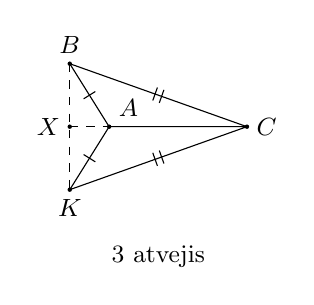
\begin{tikzpicture}[scale=.5,font=\small]
\coordinate (A) at (0,0);\coordinate (C) at (3.5,0);\coordinate (B) at (-1,1.6);\coordinate (K) at (-1,-1.6);\coordinate (X) at (-1,0);
\draw (A)--(B)--(C)--(K)--cycle (A)--(C);
\draw[dashed] (B)--(K) (X)--(A);
\path (A)--(B) node[midway,sloped,inner sep=0pt] {\krastineszymek{0}}
      (A)--(K) node[midway,sloped,inner sep=0pt] {\krastineszymek{0}}
      (B)--(C) node[midway,sloped,inner sep=0pt] {\krastineszymek{-1.25,1.25}}
      (K)--(C) node[midway,sloped,inner sep=0pt] {\krastineszymek{-1.25,1.25}};
\foreach \p/\pos in {A/above right,B/above,C/right,K/below,X/left} {\fill (\p) circle (1.6pt) node[\pos] {$\p$};}
\node at (1.25,-3.3) {3 atvejis};
\end{tikzpicture}
\end{center}
\item Įrodykite, kad $\triangle ABC=\triangle AKC$, ir išveskite, kad $\triangle ABC=\triangle DFE$. Lygybę užrašykite nurodydami atitinkamas viršūnes ta pačia tvarka.
\end{enumerate}
\end{staranchorproblem}
\begin{problem}\label{uzd:sss-breziniai-01}
Kiekviename brėžinyje raskite du lygius trikampius ir pagrįskite jų lygumą pagal tris kraštines. Atitinkamas viršūnes užrašykite ta pačia tvarka.
\begin{tasks}(1)
\task $AB=AD$, $CB=CD$.
\begin{center}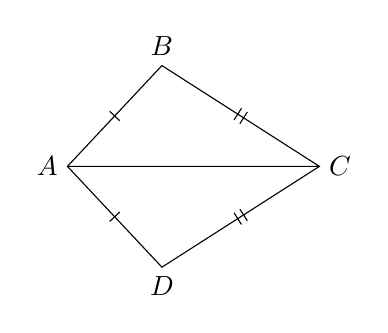
\begin{tikzpicture}[scale=.8]
\coordinate (A) at (0,0);\coordinate (C) at (4,0);\coordinate (B) at (1.5,1.6);\coordinate (D) at (1.5,-1.6);
\draw (A)--(B)--(C)--(D)--cycle (A)--(C);
\path (A)--(B) node[midway,sloped,inner sep=0pt] {\krastineszymek{0}}
      (A)--(D) node[midway,sloped,inner sep=0pt] {\krastineszymek{0}}
      (C)--(B) node[midway,sloped,inner sep=0pt] {\krastineszymek{-1.25,1.25}}
      (C)--(D) node[midway,sloped,inner sep=0pt] {\krastineszymek{-1.25,1.25}};
\foreach \p/\d in {A/left,B/above,C/right,D/below} \node[\d] at (\p) {$\p$};
\end{tikzpicture}\end{center}
\task Taškai $A,B,D$ yra vienoje tiesėje, $B$ yra tarp $A$ ir $D$; taškai $A,E,C$ yra vienoje tiesėje, $E$ yra tarp $A$ ir $C$. Duota $AB=AE$, $AC=AD$ ir $BC=DE$. Ar duomuo $BC=DE$ būtinas? Įrodykite trikampių lygumą juo nesinaudodami.
\begin{center}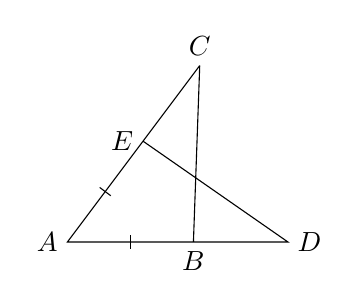
\begin{tikzpicture}[scale=.8]
\coordinate (A) at (0,0);\coordinate (B) at (2,0);\coordinate (D) at (3.5,0);\coordinate (E) at (1.2,1.6);\coordinate (C) at (2.1,2.8);
\draw (A)--(D)--(E)--(C)--cycle (B)--(C);
\path (A)--(B) node[midway,sloped,inner sep=0pt] {\krastineszymek{0}}
      (A)--(E) node[midway,sloped,inner sep=0pt] {\krastineszymek{0}};
\foreach \p/\d in {A/left,B/below,D/right,E/left,C/above} \node[\d] at (\p) {$\p$};
\end{tikzpicture}\end{center}
\task Taškai $A,B,C$ yra vienoje tiesėje, o $D,E,F$ – kitoje; $B$ yra tarp $A$ ir $C$, $E$ – tarp $D$ ir $F$. Duota $AB=DE$, $BC=EF$, $AG=DG$ ir $CG=FG$.
\begin{center}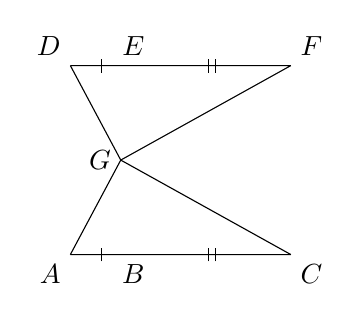
\begin{tikzpicture}[scale=.8]
\coordinate (A) at (0,0);\coordinate (B) at (1,0);\coordinate (C) at (3.5,0);\coordinate (D) at (0,3);\coordinate (E) at (1,3);\coordinate (F) at (3.5,3);\coordinate (G) at (.8,1.5);
\draw (A)--(C) (D)--(F) (A)--(G)--(C) (D)--(G)--(F);
\path (A)--(B) node[midway,sloped,inner sep=0pt] {\krastineszymek{0}}
      (D)--(E) node[midway,sloped,inner sep=0pt] {\krastineszymek{0}}
      (B)--(C) node[midway,sloped,inner sep=0pt] {\krastineszymek{-1.25,1.25}}
      (E)--(F) node[midway,sloped,inner sep=0pt] {\krastineszymek{-1.25,1.25}};
\foreach \p/\d in {A/below left,B/below,C/below right,D/above left,E/above,F/above right,G/left} \node[\d] at (\p) {$\p$};
\end{tikzpicture}\end{center}
\end{tasks}
\end{problem}

\begin{problem}\label{uzd:sss-tiesioginis-01} Duota $AB=PR$, $BC=RQ$, $CA=QP$. Užrašykite trikampių $ABC$ ir $PQR$ lygumą taip, kad viršūnės atitiktų, ir nurodykite požymį. \end{problem}
\begin{problem}\label{uzd:sss-tiesioginis-02} Atkarpos $AC$ ir $BD$ kertasi taške $O$. Duota $AB=CD$ ir $AD=CB$. Įrodykite, kad $\angle BAD=\angle DCB$, $\angle ABD=\angle CDB$ ir $\angle ADB=\angle CBD$. \end{problem}
\begin{remark*} Kai išmoksime lygiagrečių tiesių požymius, iš paskutinių dviejų lygybių gausime $AB\parallel CD$ ir $AD\parallel BC$. Tai bus lygiagretainio požymių pagrindas. \end{remark*}
\begin{starproblem}\label{uzd:sss-konstr-01} Nubraižykite atkarpą $AB$ ir tašką $C$, nepriklausantį tiesei $AB$. Kitoje tiesės $AB$ pusėje skriestuvu raskite tašką $D$, kuriam $AD=AC$, $BD=BC$. Pagrįskite, kad toks taškas egzistuoja ir kad $\triangle ABC=\triangle ABD$. Kiek tokių taškų $D$ gali būti toje pusėje? \end{starproblem}
\section{Trikampio priekampis}
\kelias{Kur einame.} Iki šiol įrodinėjome tik lygybes. Dabar pirmą kartą įrodysime kampų nelygybę. Pagrindinis įrankis – \emph{pusiaukraštinės pratęsimas dvigubai}: pratęsę pusiaukraštinę už kraštinės vidurio tiek pat, gauname naują trikampį, lygų vienai pradinio trikampio daliai, ir taip „perkeliame“ kampą į kitą vietą. Šį metodą dar panaudosime \ref{uzd:priekampis-pusiaukrastine} uždavinyje.
\Needspace{10\baselineskip}
\begin{definition}\label{apib:priekampis} Trikampio \emph{priekampis} yra kampas, gretutinis trikampio vidaus kampui. Pavyzdžiui, jei taškas $E$ yra tiesėje $AC$ už taško $C$, tai $\angle BCE$ yra trikampio $ABC$ priekampis prie viršūnės $C$.
\begin{center}
\begin{tikzpicture}[scale=.8]
\coordinate (A) at (-2,0);\coordinate (B) at (0,2);\coordinate (C) at (2,0);\coordinate (E) at (4.7,0);
\draw (A)--(E) (A)--(B)--(C);
\draw (2.5,0) arc[start angle=0,end angle=135,radius=.5];
\foreach \p/\pos in {A/left,B/above,C/below,E/right} {\fill (\p) circle (1.6pt) node[\pos] {$\p$};}
\end{tikzpicture}
\end{center}
\end{definition}
\begin{problem}\label{uzd:priekampis-supratimas} Nubrėžkite trikampį $ABC$, pratęskite $AC$ už $C$ ir pažymėkite priekampį. Kuris trikampio kampas yra jam gretutinis? Kurie du trikampio kampai nėra jam gretutiniai? \end{problem}
\begin{staranchorproblem}[Trikampio priekampio nelygybė]\label{atr:priekampis-nelygybe}
Duotas trikampis $ABC$ ir jo priekampis $BCE$: kraštinė $AC$ pratęsta už viršūnės $C$ iki taško $E$. Įrodykite, kad šis priekampis didesnis už kiekvieną jam negretutinį trikampio kampą.
\begin{center}
\begin{tikzpicture}[scale=.8]
\coordinate (A) at (-2,0);\coordinate (B) at (0,2);\coordinate (C) at (2,0);\coordinate (E) at (4.7,0);
\draw (A)--(E) (A)--(B)--(C);
\foreach \p/\pos in {A/left,B/above,C/below,E/right} {\fill (\p) circle (1.6pt);\node[\pos] at (\p) {$\p$};}
\end{tikzpicture}
\end{center}
\begin{enumerate}[label=\alph*),leftmargin=*]
\item Pažymėkite kraštinės $BC$ vidurio tašką $M$. Pratęskite atkarpą $AM$ už $M$ iki taško $D$ taip, kad $MD=MA$, ir nubrėžkite $CD$, kaip parodyta brėžinyje. Įrodykite, kad $\triangle ABM=\triangle DCM$.
\begin{center}
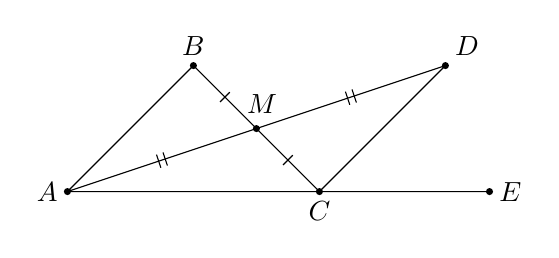
\begin{tikzpicture}[scale=.8]
\coordinate (A) at (-2,0);\coordinate (B) at (0,2);\coordinate (C) at (2,0);\coordinate (E) at (4.7,0);\coordinate (M) at (1,1);\coordinate (D) at (4,2);
\draw (A)--(E) (A)--(B)--(C)--(D) (A)--(D);
\path (B)--(M) node[midway,sloped,inner sep=0pt] {\krastineszymek{0}}
      (M)--(C) node[midway,sloped,inner sep=0pt] {\krastineszymek{0}}
      (A)--(M) node[midway,sloped,inner sep=0pt] {\krastineszymek{-1.25,1.25}}
      (M)--(D) node[midway,sloped,inner sep=0pt] {\krastineszymek{-1.25,1.25}};
\foreach \p/\pos in {A/left,B/above,C/below,E/right,D/above right} {\fill (\p) circle (1.6pt);\node[\pos] at (\p) {$\p$};}
\fill (M) circle (1.6pt) node[above=2pt,xshift=2pt] {$M$};
\end{tikzpicture}
\end{center}
\item Įrodykite, kad spindulys $CD$ eina kampo $BCE$ viduje, ir išveskite, kad $\angle BCE>\angle ABC$.
\item Panašią konstrukciją atlikite su kraštine $AC$: naujame brėžinyje pažymėkite jos vidurio tašką $N$, pratęskite $BN$ už $N$ iki taško $F$ taip, kad $NF=NB$, ir nubrėžkite $FC$. Pratęskite $FC$ už $C$ iki taško $G$, kaip parodyta brėžinyje. Įrodykite, kad $\triangle ABN=\triangle CFN$.
\begin{center}
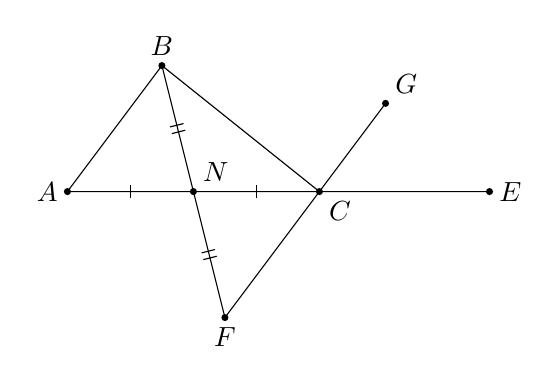
\begin{tikzpicture}[scale=.8]
\coordinate (A) at (-2,0);\coordinate (B) at (-.5,2);\coordinate (C) at (2,0);\coordinate (E) at (4.7,0);\coordinate (N) at (0,0);\coordinate (F) at (.5,-2);\coordinate (G) at (3.05,1.4);
\draw (A)--(E) (A)--(B)--(C) (B)--(F)--(G);
\path (A)--(N) node[midway,sloped,inner sep=0pt] {\krastineszymek{0}}
      (N)--(C) node[midway,sloped,inner sep=0pt] {\krastineszymek{0}}
      (B)--(N) node[midway,sloped,inner sep=0pt] {\krastineszymek{-1.25,1.25}}
      (N)--(F) node[midway,sloped,inner sep=0pt] {\krastineszymek{-1.25,1.25}};
\foreach \p/\pos in {A/left,B/above,C/below right,E/right,N/above right,F/below,G/above right}
{\fill (\p) circle (1.6pt) node[\pos] {$\p$};}
\end{tikzpicture}
\end{center}
\item Įrodykite, kad spindulys $CG$ eina kampo $BCE$ viduje, ir išveskite, kad $\angle BCE>\angle BAC$.
\item Remdamiesi b) ir d) dalių išvadomis, įrodykite, kad priekampis $BCE$ yra didesnis už kiekvieną jam negretutinį trikampio $ABC$ kampą.
\end{enumerate}
\end{staranchorproblem}
\begin{problem}\label{uzd:priekampis-pratimai} Trikampio $ABC$ priekampis prie $C$ lygus $100^\circ$. Ar kampas $A$ gali būti lygus $100^\circ$? Ar jis gali būti didesnis negu $100^\circ$? Pagrįskite. \end{problem}
\begin{problem}\label{uzd:priekampis-taikymas} Trikampio vienas kampas lygus $110^\circ$. Naudodamiesi tik priekampio nelygybe įrodykite, kad kiti du kampai yra smailieji. \end{problem}
\begin{problem}\label{uzd:priekampis-suma} Įrodykite, kad bet kurių dviejų trikampio kampų suma mažesnė už $180^\circ$. Išveskite, kad trikampyje gali būti ne daugiau kaip vienas statusis arba bukasis kampas. \end{problem}
\begin{anchorproblem}[Statmens vienatinumas]\label{atr:statmuo} Iki šiol be įrodymo rėmėmės tuo, kad per tašką, nepriklausantį tiesei, galima nubrėžti tik vieną tai tiesei statmeną tiesę. Įrodykite tai. \end{anchorproblem}
\begin{starproblem}\label{uzd:priekampis-pusiaukrastine} Trikampio $ABC$ pusiaukraštinė $AM$ yra ir kampo $BAC$ pusiaukampinė. Įrodykite, kad $AB=AC$.
\par\emph{Nurodymas.} Pratęskite pusiaukraštinę dvigubai, kaip \ref{atr:priekampis-nelygybe} uždavinio a) dalyje, ir ieškokite lygiašonio trikampio. \end{starproblem}

\section{Atkarpos vidurio statmuo}
\kelias{Kur einame.} Kur yra visi taškai, vienodai nutolę nuo dviejų duotų taškų? Atsakymą sudaro du teiginiai – savybė ir jai atvirkštinis teiginys (požymis), – ir abu įrodomi jau žinomais požymiais. Atkreipkite dėmesį, kaip skiriasi šie teiginiai ir kodėl taškus, esančius pačioje atkarpos tiesėje, tenka nagrinėti atskirai.
\Needspace{10\baselineskip}
\begin{definition}\label{apib:vidurio-statmuo} Atkarpos \emph{vidurio statmuo} yra tiesė, einanti per atkarpos vidurio tašką ir statmena tai atkarpai.
\begin{center}
\begin{tikzpicture}[scale=.8]
\coordinate (A) at (-1.5,0);\coordinate (B) at (1.5,0);\coordinate (M) at (0,0);
\draw (A)--(B) (0,-1)--(0,1.4) node[above] {$m$};
\draw (.25,0)--(.25,.25)--(0,.25);
\path (A)--(M) node[midway,sloped,inner sep=0pt] {\krastineszymek{0}}
      (M)--(B) node[midway,sloped,inner sep=0pt] {\krastineszymek{0}};
\foreach \p/\pos in {A/left,B/right,M/below left} {\fill (\p) circle (1.6pt) node[\pos] {$\p$};}
\end{tikzpicture}
\end{center}
\end{definition}
\begin{problem}\label{uzd:vidurio-supratimas-01} Atkarpos $AB$ vidurio taškas yra $M$. Tiesė $m$ eina per $M$. Kokios dar sąlygos reikia, kad $m$ būtų $AB$ vidurio statmuo? Ar tiesė, kuri statmena $AB$ taške $A$, yra $AB$ vidurio statmuo? \end{problem}
\begin{anchorproblem}[Atkarpos vidurio statmens savybė]\label{atr:vidurio-savybe} Įrodykite, jog kiekvienas atkarpos vidurio statmens taškas yra vienodai nutolęs nuo jos galų. \end{anchorproblem}
\begin{problem}\label{uzd:vidurio-savybe-01} Taškas $P$ yra atkarpos $AB$ vidurio statmenyje, $PA=8$ cm. Raskite $PB$. \end{problem}
\begin{problem}\label{uzd:vidurio-savybe-02} Atkarpos $AB$ vidurio statmuo eina per taškus $P$ ir $Q$. Įrodykite, kad $\angle APQ=\angle QPB$, jei $P\ne Q$ ir $P$ nėra tiesėje $AB$. \end{problem}
\begin{anchorproblem}[Vidurio statmens požymis]\label{atr:vidurio-atvirkstine} Įrodykite: jei taškas vienodai nutolęs nuo atkarpos galų, tai jis yra tos atkarpos vidurio statmenyje. Atskirai aptarkite atvejį, kai taškas yra pačioje tiesėje, kuriai priklauso atkarpa. \end{anchorproblem}
\begin{problem}\label{uzd:vidurio-atvirkstine-01} Žinoma, kad $XA=XB$ ir $YA=YB$, o $X\ne Y$. Įrodykite, kad tiesė $XY$ yra atkarpos $AB$ vidurio statmuo. \end{problem}
\begin{problem}\label{uzd:vidurio-taikymas-01} Atkarpos $AB$ vidurio statmenyje yra taškas $P$, nepriklausantis tiesei $AB$. Taškas $M$ yra atkarpos $AB$ vidurys, $AB=10$ cm, o trikampio $PAB$ perimetras lygus $24$ cm. Raskite $PA$, $PB$ ir $AM$. \end{problem}
\begin{problem}\label{uzd:vidurio-taikymas-02} Trikampio $ABC$ pusiaukraštinė $AM$ yra ir aukštinė. Įrodykite, kad $AB=AC$. \end{problem}
\begin{starproblem}\label{uzd:vidurio-taikymas-03} Trikampyje $ABC$ duota $AB=AC$, $M$ yra kraštinės $BC$ vidurio taškas. Kraštinių $AB$ ir $AC$ vidurio statmenys kertasi taške $O$. Įrodykite, kad $OB=OC$ ir kad taškas $O$ priklauso tiesei $AM$. \end{starproblem}
\section*{Svarbiausios temos išvados}
Prieš skaitydami pabandykite atsakyti: kaip parenkamos atitinkamos viršūnės? Kaip iš trikampių lygumo gaunama atkarpų lygybė? Kuo skiriasi savybė nuo jai atvirkštinio teiginio?
\begin{itemize}
\item Trikampiams palyginti taikome tris požymius: dvi kraštines ir kampą tarp jų; kraštinę ir du kampus prie jos; tris kraštines (\ref{atr:sss-poz}). Atitinkamas viršūnes rašome ta pačia tvarka.
\item Lygios dvi kraštinės ir bet kuris kampas savaime nesudaro pirmojo požymio: kampas turi būti tarp tų kraštinių (\ref{uzd:lygybe-ssa-01}).
\item Lygiašonio trikampio pagrindo kampai lygūs (\ref{atr:lygias-pagrindo-kampai}); jei du trikampio kampai lygūs, tai trikampis lygiašonis (\ref{atr:lygias-atvirkstine}).
\item Lygiašonio trikampio pusiaukraštinė į pagrindą yra ir aukštinė, ir pusiaukampinė (\ref{atr:lygias-pusiaukrastine}). Atvirkščiai: jei pusiaukraštinė yra pusiaukampinė (\ref{uzd:priekampis-pusiaukrastine}) arba aukštinė (\ref{uzd:vidurio-taikymas-02}), trikampis lygiašonis.
\item Trikampio priekampis didesnis už kiekvieną jam negretutinį trikampio kampą (\ref{atr:priekampis-nelygybe}). Todėl dviejų trikampio kampų suma mažesnė už $180^\circ$ (\ref{uzd:priekampis-suma}), o per tašką, nepriklausantį tiesei, eina vienintelis jai statmuo (\ref{atr:statmuo}).
\item Atkarpos vidurio statmens taškai ir tik jie vienodai nutolę nuo jos galų (\ref{atr:vidurio-savybe}, \ref{atr:vidurio-atvirkstine}).
\end{itemize}
\textbf{Metodai, kuriuos išmokome.} Papildoma linija, sukurianti lygius trikampius (pusiaukampinė lygiašoniame trikampyje). Trikampio palyginimas su juo pačiu. Du lygiašoniai trikampiai su bendru pagrindu. Pusiaukraštinės pratęsimas dvigubai. Atvejų nagrinėjimas pagal taškų išsidėstymą: brėžinys rodo tik vieną atvejį.
\section*{Atraminiai faktai: vaizdinė santrauka}
Vienodi brūkšneliai žymi lygias atkarpas, o vienodos graikiškos raidės – lygius kampus. Nuorodos nurodo atitinkamus atraminius uždavinius.

\Needspace{13\baselineskip}
\textbf{Lygiašonio trikampio savybė ir požymis} (\ref{atr:lygias-pagrindo-kampai}, \ref{atr:lygias-atvirkstine})
\begin{center}
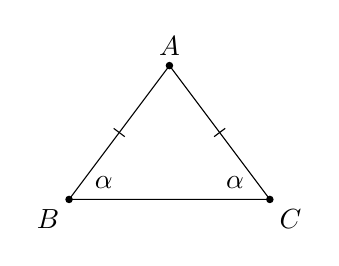
\begin{tikzpicture}[scale=.85]
\coordinate (A) at (1.5,2); \coordinate (B) at (0,0); \coordinate (C) at (3,0);
\draw (A)--(B) node[midway,sloped,inner sep=0pt] {\krastineszymek{0}}
      --(C)--(A) node[midway,sloped,inner sep=0pt] {\krastineszymek{0}};
\node at (.52,.25) {$\alpha$}; \node at (2.48,.25) {$\alpha$};
\foreach \p/\pos in {A/above,B/below left,C/below right} {\fill (\p) circle (1.6pt) node[\pos] {$\p$};}
\end{tikzpicture}
\end{center}
Jei $AB=AC$, tai $\angle ABC=\angle BCA$. Ir atvirkščiai: jei $\angle ABC=\angle BCA$, tai $AB=AC$.

\Needspace{14\baselineskip}
\textbf{Pusiaukraštinė į lygiašonio trikampio pagrindą} (\ref{atr:lygias-pusiaukrastine})
\begin{center}
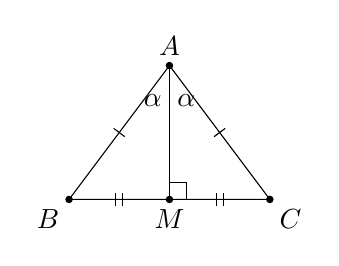
\begin{tikzpicture}[scale=.85]
\coordinate (A) at (1.5,2); \coordinate (B) at (0,0); \coordinate (C) at (3,0); \coordinate (M) at (1.5,0);
\draw (A)--(B) node[midway,sloped,inner sep=0pt] {\krastineszymek{0}}
      --(C)--(A) node[midway,sloped,inner sep=0pt] {\krastineszymek{0}};
\draw (A)--(M);
\path (B)--(M) node[midway,sloped,inner sep=0pt] {\krastineszymek{-1.25,1.25}}
      (M)--(C) node[midway,sloped,inner sep=0pt] {\krastineszymek{-1.25,1.25}};
\draw (1.5,.25)--(1.75,.25)--(1.75,0);
\node at (1.25,1.48) {$\alpha$}; \node at (1.75,1.48) {$\alpha$};
\foreach \p/\pos in {A/above,B/below left,C/below right,M/below} {\fill (\p) circle (1.6pt) node[\pos] {$\p$};}
\end{tikzpicture}
\end{center}
Jei $AB=AC$ ir $BM=MC$, tai pusiaukraštinė $AM$ yra ir aukštinė, ir kampo $BAC$ pusiaukampinė: $AM\perp BC$, $\angle BAM=\angle MAC$.

\Needspace{13\baselineskip}
\textbf{Lygiakraščio trikampio savybė ir požymis} (\ref{atr:lygiakrastis-kampai})
\begin{center}
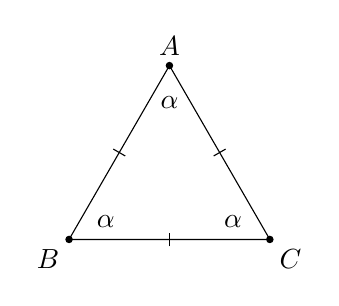
\begin{tikzpicture}[scale=.85]
\coordinate (A) at (1.5,2.598); \coordinate (B) at (0,0); \coordinate (C) at (3,0);
\draw (A)--(B) node[midway,sloped,inner sep=0pt] {\krastineszymek{0}}
      --(C) node[midway,sloped,inner sep=0pt] {\krastineszymek{0}}
      --(A) node[midway,sloped,inner sep=0pt] {\krastineszymek{0}};
\node at (1.5,2.05) {$\alpha$}; \node at (.55,.27) {$\alpha$}; \node at (2.45,.27) {$\alpha$};
\foreach \p/\pos in {A/above,B/below left,C/below right} {\fill (\p) circle (1.6pt) node[\pos] {$\p$};}
\end{tikzpicture}
\end{center}
Trikampis yra lygiakraštis tada ir tik tada, kai visi jo kampai lygūs.

\Needspace{14\baselineskip}
\textbf{Trikampių lygumo požymis pagal tris kraštines} (\ref{atr:sss-poz})
\begin{center}
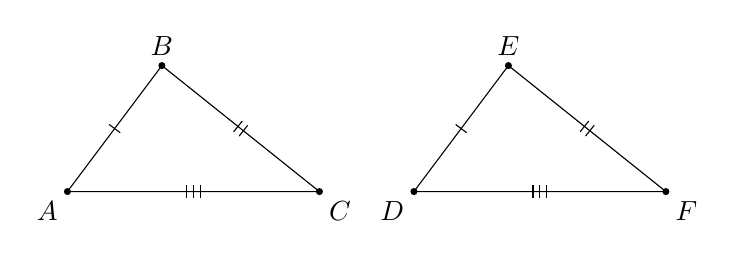
\begin{tikzpicture}[scale=.8]
\coordinate (A) at (0,0); \coordinate (B) at (1.5,2); \coordinate (C) at (4,0);
\coordinate (D) at (5.5,0); \coordinate (E) at (7,2); \coordinate (F) at (9.5,0);
\draw (A)--(B) node[midway,sloped,inner sep=0pt] {\krastineszymek{0}}
      --(C) node[midway,sloped,inner sep=0pt] {\krastineszymek{-1.25,1.25}}
      --(A) node[midway,sloped,inner sep=0pt] {\krastineszymek{-2.5,0,2.5}};
\draw (D)--(E) node[midway,sloped,inner sep=0pt] {\krastineszymek{0}}
      --(F) node[midway,sloped,inner sep=0pt] {\krastineszymek{-1.25,1.25}}
      --(D) node[midway,sloped,inner sep=0pt] {\krastineszymek{-2.5,0,2.5}};
\foreach \p/\pos in {A/below left,B/above,C/below right,D/below left,E/above,F/below right} {\fill (\p) circle (1.6pt) node[\pos] {$\p$};}
\end{tikzpicture}
\end{center}
Jei $AB=DE$, $BC=EF$ ir $AC=DF$, tai $\triangle ABC=\triangle DEF$. Atitinkamos viršūnės rašomos ta pačia tvarka.

\Needspace{13\baselineskip}
\textbf{Trikampio priekampio nelygybė} (\ref{atr:priekampis-nelygybe})
\begin{center}
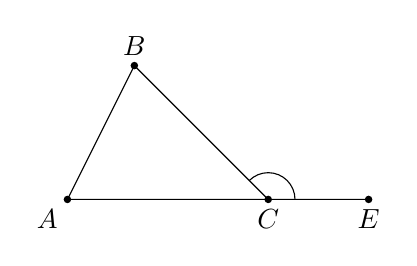
\begin{tikzpicture}[scale=.85]
\coordinate (A) at (0,0); \coordinate (B) at (1,2); \coordinate (C) at (3,0); \coordinate (E) at (4.5,0);
\draw (A)--(B)--(C)--(E) (A)--(C);
\draw (3.4,0) arc[start angle=0,end angle=135,radius=.4];
\foreach \p/\pos in {A/below left,B/above,C/below,E/below} {\fill (\p) circle (1.6pt) node[\pos] {$\p$};}
\end{tikzpicture}
\end{center}
Priekampis $\angle BCE$ yra didesnis už kiekvieną jam negretutinį trikampio kampą:
$\angle BCE>\angle BAC$ ir $\angle BCE>\angle ABC$.

\Needspace{14\baselineskip}
\textbf{Atkarpos vidurio statmens savybė ir požymis} (\ref{atr:vidurio-savybe}, \ref{atr:vidurio-atvirkstine})
\begin{center}
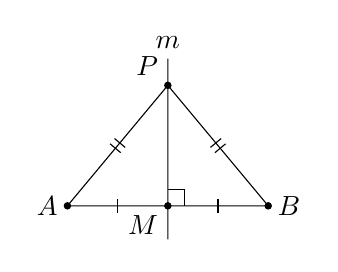
\begin{tikzpicture}[scale=.85]
\coordinate (A) at (0,0); \coordinate (B) at (3,0); \coordinate (M) at (1.5,0); \coordinate (P) at (1.5,1.8);
\draw (A)--(B) (1.5,-.5)--(1.5,2.2) node[above] {$m$} (A)--(P)--(B);
\draw (1.5,.25)--(1.75,.25)--(1.75,0);
\path (A)--(M) node[midway,sloped,inner sep=0pt] {\krastineszymek{0}}
      (M)--(B) node[midway,sloped,inner sep=0pt] {\krastineszymek{0}}
      (A)--(P) node[midway,sloped,inner sep=0pt] {\krastineszymek{-1.25,1.25}}
      (B)--(P) node[midway,sloped,inner sep=0pt] {\krastineszymek{-1.25,1.25}};
\foreach \p/\pos in {A/left,B/right,M/below left,P/above left} {\fill (\p) circle (1.6pt) node[\pos] {$\p$};}
\end{tikzpicture}
\end{center}
Jei $m$ yra $AB$ vidurio statmuo, tai kiekvienam $P\in m$ galioja $PA=PB$. Ir atvirkščiai: jei $PA=PB$, tai $P\in m$. Tai galioja ir tada, kai $P=M$.

\section*{Savikontrolė}
\setcounter{theorem}{0}\renewcommand{\thetheorem}{S\arabic{theorem}}\renewcommand{\theHtheorem}{S\arabic{theorem}}
Spręskite nežiūrėdami į ankstesnius skyrius.
\begin{problem}\label{uzd:savikontrole-01} Atkarpos $AD$ ir $BC$ kertasi taške $O$, $AO=OD$, $BO=OC$. Įrodykite, kad $AC=DB$ ir $\angle ACB=\angle DBC$. \end{problem}
\begin{problem}\label{uzd:savikontrole-02} Trikampyje $XYZ$ žinoma $XY=XZ$, $\angle XYZ=4t+3^\circ$, $\angle YZX=5t-9^\circ$. Raskite $t$ ir šiuos kampus. \end{problem}
\begin{problem}\label{uzd:savikontrole-03} Taškas $M$ yra atkarpos $AB$ vidurys, o taškas $P$ tenkina lygybę $PA=PB$. Ar teisinga, kad tiesė $PM$ yra atkarpos $AB$ vidurio statmuo? Paaiškinkite. \end{problem}
\begin{problem}\label{uzd:savikontrole-04} Trikampyje $ABC$ duota $\angle ABC=\angle ACB$, o taškai $D$ ir $E$ yra kraštinėje $BC$, $BD=CE$. Įrodykite, kad $AD=AE$. \end{problem}
\begin{problem}\label{uzd:savikontrole-05} Trikampio $ABC$ aukštinė $AH$ yra ir kampo $BAC$ pusiaukampinė. Įrodykite, kad $AB=AC$ ir $BH=HC$. \end{problem}
\begin{problem}\label{uzd:savikontrole-06} Lygiakraščio trikampio $ABC$ kraštinių $AB$, $BC$, $CA$ vidiniuose taškuose $K$, $L$, $M$ pažymėti taip, kad $AK=BL=CM$. Įrodykite, kad trikampis $KLM$ lygiakraštis. \end{problem}
\begin{problem}\label{uzd:savikontrole-07} Trikampiuose $ABC$ ir $PQR$ duota $AB=QR$, $BC=RP$ ir $AC=QP$. Ar trikampiai lygūs? Jei taip, užrašykite jų lygybę tinkama viršūnių tvarka ir nurodykite kampą, atitinkantį $\angle ABC$. \end{problem}
\begin{problem}\label{uzd:savikontrole-08} Trikampio $ABC$ kraštinė $AC$ pratęsta už $C$ iki taško $E$. Žinoma, kad $\angle BCE=110^\circ$. Kokias nelygybes galima užrašyti palyginus šį priekampį su kampais $BAC$ ir $ABC$? Pagrįskite. \end{problem}
\begin{problem}\label{uzd:savikontrole-09} Taškas $M$ yra atkarpos $AB$ vidurys, o tiesė $m$ yra šios atkarpos vidurio statmuo. Taškas $P$ priklauso tiesei $m$, o taškas $Q$ tenkina lygybę $QA=QB$. Ką galima pasakyti apie $PA$ ir $PB$? Ar $Q$ būtinai priklauso tiesei $m$? Ar išvada apie $Q$ galioja, jei $Q$ yra tiesėje $AB$? Pagrįskite. \end{problem}
\begin{problem}\label{uzd:savikontrole-10} Taškas $P$, skirtingas nuo $A$, yra kampo $XAY$ pusiaukampinėje, o taškai $B$ ir $C$ – atitinkamai kampo kraštinėse $AX$ ir $AY$, be to, $AB=AC$. Įrodykite, kad $PB=PC$. \end{problem}
\begin{problem}\label{uzd:savikontrole-11} Trikampyje $ABC$ duota $AB=AC$. Taškas $D$ yra kraštinės $AB$, o taškas $E$ – kraštinės $AC$ vidinis taškas, $AD=AE$. Įrodykite, kad $BE=CD$. \end{problem}
\begin{problem}\label{uzd:savikontrole-12} Lygiašonio trikampio perimetras yra $30$ cm, o viena kraštinė lygi $7$ cm. Raskite likusias dvi kraštines. \end{problem}
\section*{Atsakymai}
\textbf{\ref{uzd:lygybe-atitikimas-01}.} $PQ$, $PR$; $\angle PQR$, $\angle QPR$; $BC=QR$, $\angle ACB=\angle PRQ$.\par
\textbf{\ref{uzd:lygybe-sas-01}.} $BC=ED$.\par
\textbf{\ref{uzd:lygybe-asa-01}.} $AC=KM$.\par
\textbf{\ref{uzd:lygybe-ssa-01}.} Ne.\par
\textbf{\ref{uzd:lygias-perimetras-01}.} $7$ cm ir $7$ cm arba $6$ cm ir $8$ cm.\par
\textbf{\ref{uzd:lygias-kampai-01}.} $38^\circ$; ne.\par
\textbf{\ref{uzd:lygias-kampai-02}.} $x=15$, abu kampai po $40^\circ$.\par
\textbf{\ref{uzd:lygias-atvirkstine-01}.} $7$ cm.\par
\textbf{\ref{uzd:lygias-atvirkstine-02}.} $KM=LM$.\par
\textbf{\ref{uzd:lygias-pusiaukrastine-01}.} $27^\circ$ ir $90^\circ$.\par
\textbf{\ref{uzd:sss-tiesioginis-01}.} $\triangle ABC=\triangle PRQ$.\par
\textbf{\ref{uzd:sss-konstr-01}.} Vienas.\par
\textbf{\ref{uzd:priekampis-pratimai}.} Ne; ne.\par
\textbf{\ref{uzd:vidurio-savybe-01}.} $8$ cm.\par
\textbf{\ref{uzd:vidurio-taikymas-01}.} $PA=PB=7$ cm, $AM=5$ cm.\par
\textbf{\ref{uzd:savikontrole-02}.} $t=12$, abu kampai po $51^\circ$.\par
\textbf{\ref{uzd:savikontrole-03}.} Taip, jei $P\ne M$; kai $P=M$, tiesė $PM$ neapibrėžta.\par
\textbf{\ref{uzd:savikontrole-07}.} Taip, $\triangle ABC=\triangle QRP$; $\angle QRP$.\par
\textbf{\ref{uzd:savikontrole-08}.} $\angle BAC<110^\circ$, $\angle ABC<110^\circ$.\par
\textbf{\ref{uzd:savikontrole-09}.} $PA=PB$; taip; taip.\par
\textbf{\ref{uzd:savikontrole-12}.} $11{,}5$ cm ir $11{,}5$ cm.\par
\section*{Sprendimai ir įrodymai}
\begin{solution}[\ref{uzd:breziniai-lygumas-01}]
\textbf{(1)} $AO=CO$ ir $\angle BAO=\angle DCO$ (duota); $\angle AOB=\angle COD$ (kryžminiai kampai). Šie kampai yra prie kraštinių $AO$ ir $CO$, todėl $\triangle AOB=\triangle COD$ pagal kraštinę ir du kampus prie jos.\par
\textbf{(2)} $AO=CO$ ir $BO=DO$ (duota); $\angle AOB=\angle COD$ (kryžminiai kampai). Šie kampai yra tarp nurodytų atitinkamų kraštinių, todėl $\triangle AOB=\triangle COD$ pagal dvi kraštines ir kampą tarp jų.\par
\textbf{(3)} $AC=AD$ ir $\angle CAB=\angle DAB$ (duota); $AB$ – bendra kraštinė. Lygūs kampai yra tarp nurodytų atitinkamų kraštinių, todėl $\triangle CAB=\triangle DAB$ pagal dvi kraštines ir kampą tarp jų.\par
\textbf{(4)} $\angle CAB=\angle DAB$ ir $\angle ABC=\angle ABD$ (duota); $AB$ – bendra kraštinė. Nurodyti kampai yra prie kraštinės $AB$, todėl $\triangle CAB=\triangle DAB$ pagal kraštinę ir du kampus prie jos.\par
\textbf{(5)} $AB=AE$ ir $AC=AD$ (duota). Spindulys $AB$ sutampa su $AD$, o $AC$ – su $AE$, todėl $\angle BAC=\angle EAD$: tai tas pats kampas. Jis yra tarp nurodytų atitinkamų kraštinių, todėl $\triangle ABC=\triangle AED$ pagal dvi kraštines ir kampą tarp jų.\par
\end{solution}
\begin{solution}[\ref{uzd:lygybe-atitikimas-01}] Pagal viršūnių atitikimą $A\leftrightarrow P$, $B\leftrightarrow Q$, $C\leftrightarrow R$ gauname atsakymuose nurodytas lygybes. Be jų, $AB=PQ$, $AC=PR$, $\angle ABC=\angle PQR$ ir $\angle BAC=\angle QPR$. \end{solution}
\begin{solution}[\ref{uzd:lygybe-sas-01}] Duotos dvi atitinkamos kraštinės ir kampas tarp jų, todėl $\triangle ABC=\triangle FED$ pagal dvi kraštines ir kampą tarp jų. Atitinkamos kraštinės $BC$ ir $ED$ lygios. \end{solution}
\begin{solution}[\ref{uzd:lygybe-asa-01}] Prie lygių kraštinių $AB$ ir $KL$ esantys atitinkami kampai lygūs. Todėl $\triangle ABC=\triangle KLM$ pagal kraštinę ir du kampus prie jos, taigi $AC=KM$. \end{solution}
\begin{solution}[\ref{uzd:lygybe-klaida-01}] Kampas $ABC$ nėra kampas tarp kraštinių $AB$ ir $AC$: tarp jų yra kampas $BAC$. Papildomai žinant $\angle BAC=\angle EDF$, požymį pagal dvi kraštines ir kampą tarp jų taikyti galima. Kad vien pradinių duomenų nepakanka, rodo \ref{uzd:lygybe-ssa-01} uždavinys. \end{solution}
\begin{solution}[\ref{uzd:lygybe-ssa-01}] Kraštinė $AB$ abiem trikampiams bendra, $AC=AD$ pagal konstrukciją, o $\angle ABC=\angle ABD$, nes taškas $D$ yra spindulyje $BC$: tai tas pats kampas. Tačiau $D$ yra tarp $C$ ir $B$, todėl $BC=BD+DC>BD$. Trikampių atitinkamos kraštinės nelygios, taigi trikampiai nelygūs. Vadinasi, dviejų kraštinių ir ne tarp jų esančio kampo lygybės nepakanka. \end{solution}
\begin{solution}[\ref{uzd:lygybe-susikirtimas-01}] $AO=OC$, $BO=OD$, o $\angle AOB=\angle COD$ kaip kryžminiai kampai. Todėl $\triangle AOB=\triangle COD$ pagal dvi kraštines ir kampą tarp jų; iš čia $AB=CD$, $\angle ABO=\angle CDO$ ir $\angle BAO=\angle DCO$. Lygiai taip pat $\angle AOD=\angle COB$ (kryžminiai), todėl $\triangle AOD=\triangle COB$ pagal dvi kraštines ir kampą tarp jų, taigi $AD=CB$.\par
Kitos poros. Taškas $O$ yra atkarpoje $BD$, todėl $\angle ABD=\angle ABO=\angle CDO=\angle CDB$. Be to, $AB=CD$, o $BD$ bendra. Todėl $\triangle ABD=\triangle CDB$ pagal dvi kraštines ir kampą tarp jų. Analogiškai $O$ yra atkarpoje $AC$, todėl $\angle BAC=\angle BAO=\angle DCO=\angle DCA$; kadangi $AB=CD$ ir $AC$ bendra, $\triangle BAC=\triangle DCA$ pagal dvi kraštines ir kampą tarp jų. \end{solution}
\begin{solution}[\ref{uzd:lygybe-pusiaukampine-01}] $AB=AC$, $AD$ bendra, $\angle BAD=\angle DAC$. Taigi $\triangle BAD=\triangle CAD$ pagal dvi kraštines ir kampą tarp jų. Todėl $BD=DC$, o kampai $ADB$ ir $ADC$ lygūs. Jie gretutiniai, vadinasi, kiekvienas statusis ir $AD\perp BC$. \end{solution}
\begin{solution}[\ref{uzd:lygias-supratimas-01}] Pagrindas $BC$, kampai prie jo – $\angle ABC$ ir $\angle BCA$. Jei lygios visos kraštinės, tai lygios ir bet kurios dvi iš jų, todėl trikampis atitinka apibrėžimą, o pagrindu galima laikyti bet kurią kraštinę. \end{solution}
\begin{solution}[\ref{uzd:lygias-perimetras-01}]
Jei $6$ cm ilgio kraštinė yra pagrindas, tai abi šoninės kraštinės lygios $(20-6):2=7$ cm.\par
Jei $6$ cm ilgio kraštinė yra šoninė, tai kita šoninė kraštinė taip pat lygi $6$ cm, o pagrindas lygus $20-6-6=8$ cm.\par
Abiem atvejais gauti kraštinių ilgiai tenkina trikampio nelygybę ($6<7+7$; $8<6+6$), todėl abu atsakymai galimi.
\end{solution}
\begin{solution}[\ref{atr:lygias-pagrindo-kampai}] Tarkime, $AB=AC$, o kampo $BAC$ pusiaukampinė kerta $BC$ taške $D$ (ji eina kampo viduje, todėl kerta atkarpą $BC$). Kaip \ref{uzd:lygybe-pusiaukampine-01} uždavinyje, $\triangle BAD=\triangle CAD$ pagal dvi kraštines ir kampą tarp jų. Atitinkami kampai $\angle ABC$ ir $\angle BCA$ lygūs. \end{solution}
\begin{solution}[\ref{uzd:lygias-kampai-01}] Pagal lygiašonio trikampio kampų prie pagrindo savybę (\ref{atr:lygias-pagrindo-kampai}) $\angle ACB=38^\circ$. Lygybė $AB=BC$ neišplaukia. Nubraižykime $38^\circ$ kampą su viršūne $B$ ir vienoje jo kraštinėje atidėkime $BA=3$ cm. Apskritimas, kurio centras $A$ ir spindulys $3$ cm, antrą kartą kerta kitą kampo kraštinę taške $C$. Tada $AB=AC$ ir $\angle ABC=38^\circ$, tačiau išmatavę gauname $BC\approx4{,}7$ cm $\ne AB$.
\begin{remark*} Įrodyti, kad $AB\ne BC$, remiantis vien šio lapo faktais, nepavyktų: tam reikia trikampio kampų sumos. Todėl čia užtenka konstrukcijos ir matavimo. \end{remark*}
\end{solution}
\begin{solution}[\ref{uzd:lygias-kampai-02}] Kampai prie pagrindo $PR$ lygūs, todėl $2x+10=3x-5$, $x=15$. Kiekvienas kampas lygus $40^\circ$. \end{solution}
\begin{solution}[\ref{atr:lygias-atvirkstine}] Tarkime, $\angle ABC=\angle BCA$. Palyginkime trikampius $ABC$ ir $ACB$, t.\,y. tą patį trikampį, kurio viršūnės surašytos kita tvarka. Kraštinė $BC$ abiem trikampiams bendra, o kampai prie jos poromis lygūs pagal sąlygą: $\angle ABC=\angle ACB$ ir $\angle BCA=\angle CBA$. Todėl $\triangle ABC=\triangle ACB$ pagal kraštinę ir du kampus prie jos. Vadinasi, atitinkamos kraštinės $AB$ ir $AC$ lygios. \end{solution}
\begin{solution}[\ref{uzd:lygias-atvirkstine-01}] Pagal lygiašonio trikampio požymį (\ref{atr:lygias-atvirkstine}) $AC=AB=7$ cm. \end{solution}
\begin{solution}[\ref{uzd:lygias-atvirkstine-02}] Prieš kampą $KLM$ yra kraštinė $KM$, o prieš kampą $LKM$ – kraštinė $LM$. Pagal lygiašonio trikampio požymį (\ref{atr:lygias-atvirkstine}) $KM=LM$.\par
Kampai $K$ ir $M$ nebūtinai lygūs. Nubraižykime $KL=4$ cm ir jos galuose į vieną pusę atidėkime po $30^\circ$ kampus; spinduliai susikerta taške $M$. Jei būtų $\angle K=\angle M$, tai pagal tą patį lygiašonio trikampio požymį būtų $LM=KL=4$ cm. Tačiau išmatavę gauname $LM\approx2{,}3$ cm. \end{solution}
\begin{solution}[\ref{atr:lygias-pusiaukrastine}] Pagal lygiašonio trikampio kampų prie pagrindo savybę (\ref{atr:lygias-pagrindo-kampai}) $\angle ABM=\angle MCA$. Be to, $AB=AC$, $BM=MC$. Todėl $\triangle ABM=\triangle ACM$ pagal dvi kraštines ir kampą tarp jų. Vadinasi, $\angle BAM=\angle MAC$, taigi $AM$ yra pusiaukampinė. Gretutiniai kampai $AMB$ ir $AMC$ lygūs, todėl jie statieji, o $AM$ yra aukštinė. \end{solution}
\begin{solution}[\ref{uzd:lygias-pusiaukrastine-01}] Pagal lygiašonio trikampio pusiaukraštinės į pagrindą savybę (\ref{atr:lygias-pusiaukrastine}) $\angle MAC=\angle BAM=27^\circ$, o $\angle AMB=90^\circ$. \end{solution}
\begin{solution}[\ref{uzd:lygias-aukstine-01}] Pažymėkime $BC$ vidurio tašką $M$. Pagal lygiašonio trikampio pusiaukraštinės į pagrindą savybę (\ref{atr:lygias-pusiaukrastine}) $AM\perp BC$, o pagal sąlygą $AD\perp BC$. Per tašką $A$ eina tik viena tiesei $BC$ statmena tiesė, todėl tiesės $AM$ ir $AD$ sutampa. Ši tiesė su $BC$ turi vieną bendrą tašką, vadinasi, $D=M$. Dabar $BD=DC$, o pagal tą pačią pusiaukraštinės savybę $\angle BAD=\angle DAC$. \end{solution}
\begin{solution}[\ref{uzd:lygias-pusiaukampines-01}] Pagal lygiašonio trikampio kampų prie pagrindo savybę (\ref{atr:lygias-pagrindo-kampai}) $\angle ABC=\angle ACB$, todėl jų pusės taip pat lygios: $\angle DBC=\angle ECB$. Palyginkime trikampius $DBC$ ir $ECB$: kraštinė $BC$ bendra, $\angle DBC=\angle ECB$, $\angle DCB=\angle EBC$. Todėl $\triangle DBC=\triangle ECB$ pagal kraštinę ir du kampus prie jos, taigi $BD=CE$. \end{solution}
\begin{solution}[\ref{uzd:lygiakrastis-supratimas-01}] Taip, lygiakraščiame trikampyje bent dvi kraštinės lygios. Ne kiekvienas lygiašonis yra lygiakraštis: pavyzdžiui, galima nubraižyti lygiašonį trikampį, kurio pagrindas trumpesnis už šonines kraštines. \end{solution}
\begin{solution}[\ref{atr:lygiakrastis-kampai}] Jei $AB=AC=BC$, lyginant poromis lygias kraštines pagal lygiašonio trikampio kampų prie pagrindo savybę (\ref{atr:lygias-pagrindo-kampai}) gauname, kad visi kampai lygūs. Jei visi kampai lygūs, taikydami lygiašonio trikampio požymį (\ref{atr:lygias-atvirkstine}) kampų poroms gauname $AB=AC=BC$. \end{solution}
\begin{solution}[\ref{uzd:lygiakrastis-kampai-01}] Kampai lygūs pagal lygiakraščio trikampio savybę (\ref{atr:lygiakrastis-kampai}). Vien iš jų lygybės dydžio $60^\circ$ nenustatome: reikia papildomo fakto apie trikampio kampų sumą. \end{solution}
\begin{solution}[\ref{atr:sss-poz}]
\textbf{a)} Pagal konstrukciją $AK=DF$ ir $\angle CAK=\angle EDF$, o pagal sąlygą $AC=DE$. Todėl $\triangle AKC=\triangle DFE$ pagal dvi kraštines ir kampą tarp jų, taigi $KC=FE$. Vadinasi, $AK=DF=AB$ ir $CK=FE=CB$.

\textbf{b)} Pagal a) dalį trikampiai $ABK$ ir $CBK$ (jei jie neišsigimę) yra lygiašoniai su bendru pagrindu $BK$, todėl $\angle ABK=\angle AKB$ ir $\angle CBK=\angle CKB$.

\emph{1 atvejis: $X$ yra tarp $A$ ir $C$.} Spindulys $BK$ eina kampo $ABC$ viduje, o spindulys $KB$ – kampo $AKC$ viduje. Todėl
\[
\angle ABC=\angle ABK+\angle KBC=\angle AKB+\angle BKC=\angle AKC.
\]

\emph{2 atvejis: $X=A$} (atvejis $X=C$ nagrinėjamas analogiškai). Tada $A$ yra atkarpoje $BK$, todėl $\angle ABC=\angle KBC$ ir $\angle AKC=\angle BKC$. Šie kampai lygūs kaip lygiašonio trikampio $CBK$ kampai prie pagrindo.

\emph{3 atvejis: $X$ yra už atkarpos $AC$}, pavyzdžiui, $A$ yra tarp $X$ ir $C$ (kitas atvejis analogiškas). Tada spindulys $BA$ eina kampo $XBC$ viduje, o spindulys $BX$ sutampa su $BK$. Todėl $\angle ABC=\angle XBC-\angle XBA=\angle KBC-\angle KBA$. Lygiai taip pat $\angle AKC=\angle BKC-\angle BKA$. Kadangi $\angle KBC=\angle BKC$ ir $\angle KBA=\angle BKA$, gauname $\angle ABC=\angle AKC$.

\textbf{c)} $AB=AK$, $BC=KC$, o kampai tarp šių kraštinių $\angle ABC$ ir $\angle AKC$ lygūs pagal b) dalį. Todėl $\triangle ABC=\triangle AKC$ pagal dvi kraštines ir kampą tarp jų. Pagal a) dalį $\triangle AKC=\triangle DFE$. Vadinasi, trikampio $ABC$ kraštinės ir kampai lygūs atitinkamiems trikampio $DFE$ elementams: $\triangle ABC=\triangle DFE$.
\end{solution}
\begin{solution}[\ref{uzd:sss-breziniai-01}]
\textbf{(1)} $AB=AD$, $CB=CD$ pagal sąlygą, o $AC$ yra bendra kraštinė. Todėl $\triangle ABC=\triangle ADC$ pagal tris kraštines.\par
\textbf{(2)} $AB=AE$, $AC=AD$ ir $BC=ED$ pagal sąlygą, todėl $\triangle ABC=\triangle AED$ pagal tris kraštines. Duomuo $BC=DE$ nebūtinas: $\angle BAC=\angle EAD$ (tas pats kampas), todėl $\triangle ABC=\triangle AED$ pagal dvi kraštines ir kampą tarp jų, kaip \ref{uzd:breziniai-lygumas-01}(5) uždavinyje, o lygybė $BC=ED$ iš to išplaukia.\par
\textbf{(3)} Kadangi $B$ ir $E$ yra atitinkamų atkarpų vidiniai taškai, $AC=AB+BC=DE+EF=DF$. Pagal sąlygą $AG=DG$ ir $CG=FG$, todėl $\triangle ACG=\triangle DFG$ pagal tris kraštines.
\end{solution}
\begin{solution}[\ref{uzd:sss-tiesioginis-01}] Iš duotų lygybių atitinka $A\leftrightarrow P$, $B\leftrightarrow R$, $C\leftrightarrow Q$. Pagal tris kraštines $\triangle ABC=\triangle PRQ$. \end{solution}
\begin{solution}[\ref{uzd:sss-tiesioginis-02}] $AB=CD$, $AD=CB$, o $BD$ yra bendra. Todėl $\triangle BAD=\triangle DCB$ pagal tris kraštines (atitinka $B\leftrightarrow D$, $A\leftrightarrow C$, $D\leftrightarrow B$). Atitinkami kampai lygūs: $\angle BAD=\angle DCB$, $\angle ABD=\angle CDB$, $\angle ADB=\angle CBD$. \end{solution}
\begin{solution}[\ref{uzd:sss-konstr-01}] Nubrėžkite apskritimus, kurių centrai $A$, $B$, o spinduliai atitinkamai $AC$, $BC$. Vienas jų susikirtimo taškas yra $C$; kitoje $AB$ pusėje pasirinkite susikirtimo tašką $D$.\par
\emph{Egzistavimas.} Kitoje tiesės $AB$ pusėje atidėkime kampą $BAD$, lygų kampui $BAC$, ir jo kraštinėje atkarpą $AD=AC$. Kadangi $AB$ bendra, $\triangle ABC=\triangle ABD$ pagal dvi kraštines ir kampą tarp jų, todėl $BD=BC$. Taigi toks taškas $D$ egzistuoja, o $\triangle ABC=\triangle ABD$ (taip pat ir pagal tris kraštines).\par
\emph{Vienatinumas.} Jei toje pačioje $AB$ pusėje būtų kitas toks taškas $D'$, pagal trijų kraštinių požymį $\triangle ABD=\triangle ABD'$. Todėl $\angle BAD=\angle BAD'$, o kampas į tą pačią tiesės pusę atidedamas vieninteliu būdu, taigi spinduliai $AD$ ir $AD'$ sutampa. Kadangi $AD=AD'$, sutampa ir taškai $D$ bei $D'$. \end{solution}
\begin{solution}[\ref{uzd:priekampis-supratimas}] Jei $E$ yra tiesėje $AC$ už $C$, priekampis yra $\angle BCE$. Jam gretutinis $\angle BCA$, o negretutiniai – $\angle BAC$ ir $\angle ABC$. \end{solution}
\begin{solution}[\ref{atr:priekampis-nelygybe}]
\textbf{a)} Pagal konstrukciją $BM=CM$ ir $AM=DM$, o $\angle AMB=\angle DMC$ kaip kryžminiai kampai. Todėl $\triangle ABM=\triangle DCM$ pagal dvi kraštines ir kampą tarp jų. Atitinkami kampai lygūs: $\angle ABC=\angle MCD$.

\textbf{b)} Taškai $M$ ir $D$ priklauso tam pačiam spinduliui iš $A$, todėl yra toje pačioje tiesės $AC$ (ji sutampa su tiese $CE$) pusėje; toje pačioje pusėje yra ir $B$, nes $M$ yra atkarpoje $BC$. Atkarpa $AD$ kerta tiesę $BC$ taške $M$, todėl $A$ ir $D$ yra skirtingose tiesės $BC$ pusėse; $A$ ir $E$ taip pat yra skirtingose pusėse, nes $C$ yra tarp jų. Vadinasi, $D$ ir $E$ yra toje pačioje tiesės $BC$ pusėje. Taigi spindulys $CD$ eina kampo $BCE$ viduje ir $\angle MCD<\angle BCE$. Pagal a) dalį $\angle ABC=\angle MCD$, todėl $\angle ABC<\angle BCE$.

\textbf{c)} $AN=CN$, $BN=FN$, o $\angle ANB=\angle CNF$ kaip kryžminiai kampai. Todėl $\triangle ABN=\triangle CFN$ pagal dvi kraštines ir kampą tarp jų, taigi $\angle BAC=\angle FCN$.

\textbf{d)} Kampai $FCN$ ir $GCE$ yra kryžminiai, todėl $\angle FCN=\angle GCE$. Atkarpa $BF$ kerta tiesę $AC$ taške $N$, o atkarpa $FG$ – taške $C$; todėl ir $B$, ir $G$ yra kitoje tiesės $AC$ pusėje nei $F$, t.\,y. toje pačioje pusėje. Taškai $F$ ir $N$ priklauso tam pačiam spinduliui iš $B$, o $N$ yra atkarpoje $AC$, todėl $F$, $N$ ir $A$ yra toje pačioje tiesės $BC$ pusėje. Kadangi $C$ yra tarp $F$ ir $G$ bei tarp $A$ ir $E$, taškai $G$ ir $E$ abu yra kitoje tiesės $BC$ pusėje, t.\,y. toje pačioje. Vadinasi, spindulys $CG$ eina kampo $BCE$ viduje ir $\angle GCE<\angle BCE$. Pagal c) dalį $\angle BAC=\angle FCN=\angle GCE$, taigi $\angle BAC<\angle BCE$.

\textbf{e)} Pagal b) dalį $\angle BCE>\angle ABC$, o pagal d) dalį $\angle BCE>\angle BAC$. Tai abu trikampio kampai, negretutiniai priekampiui $BCE$, todėl jis didesnis už kiekvieną iš jų.
\end{solution}
\begin{solution}[\ref{uzd:priekampis-pratimai}] Ne: pagal trikampio priekampio nelygybę (\ref{atr:priekampis-nelygybe}) kampas $A$ yra griežtai mažesnis už $100^\circ$, todėl negali nei jam prilygti, nei jo viršyti. \end{solution}
\begin{solution}[\ref{uzd:priekampis-taikymas}] Tarkime, $\angle A=110^\circ$. Priekampis prie $B$ yra didesnis už $\angle A$, todėl $180^\circ-\angle B>110^\circ$ ir $\angle B<70^\circ$. Taip pat $\angle C<70^\circ$. Abu kampai smailieji. \end{solution}
\begin{solution}[\ref{uzd:priekampis-suma}] Tarkime, $\angle A$ ir $\angle C$ – du trikampio $ABC$ kampai. Priekampis prie $C$ lygus $180^\circ-\angle C$ ir pagal trikampio priekampio nelygybę (\ref{atr:priekampis-nelygybe}) didesnis už $\angle A$. Todėl $\angle A+\angle C<180^\circ$. Jei trikampyje būtų du nesmailieji kampai, jų suma būtų ne mažesnė už $180^\circ$, o tai neįmanoma. \end{solution}
\begin{solution}[\ref{atr:statmuo}] Tarkime priešingai: per tašką $P$, nepriklausantį tiesei $l$, eina dvi skirtingos tiesės, statmenos $l$. Jos kerta $l$ skirtinguose taškuose $H$ ir $K$: jei kirstų tame pačiame taške, tame taške į tą pačią tiesės pusę būtų atidėti du skirtingi statieji kampai. Pratęskime $HK$ už $K$ iki taško $T$. Trikampio $PHK$ priekampis $PKT$ yra gretutinis stačiajam kampui $PKH$, todėl lygus $90^\circ$. Bet ir $\angle PHK=90^\circ$, o pagal trikampio priekampio nelygybę (\ref{atr:priekampis-nelygybe}) priekampis turėtų būti didesnis už $\angle PHK$. Gavome prieštarą.\par
 \end{solution}
\begin{solution}[\ref{uzd:priekampis-pusiaukrastine}] Pratęskime $AM$ už $M$ iki taško $D$ taip, kad $MD=MA$. Kaip priekampio nelygybės įrodymo (\ref{atr:priekampis-nelygybe}) a) dalyje, $\triangle ABM=\triangle DCM$ pagal dvi kraštines ir kampą tarp jų, todėl $AB=DC$ ir $\angle BAM=\angle CDM$. Trikampyje $ACD$ turime $\angle CAD=\angle MAC=\angle BAM=\angle CDM=\angle CDA$. Pagal lygiašonio trikampio požymį (\ref{atr:lygias-atvirkstine}) $AC=DC$. Taigi $AC=DC=AB$. \end{solution}
\begin{solution}[\ref{uzd:vidurio-supratimas-01}] Reikia, kad $m\perp AB$. Tiesė, statmena $AB$ taške $A$, kerta tiesę $AB$ tik taške $A$, nes dvi skirtingos tiesės turi ne daugiau kaip vieną bendrą tašką. Kadangi $M\ne A$, ši tiesė neina per $M$, todėl nėra vidurio statmuo. \end{solution}
\begin{solution}[\ref{atr:vidurio-savybe}] Tarkime, $M$ – $AB$ vidurys, o $P$ – vidurio statmens taškas. Jei $P=M$, tai $PA=PB$ pagal vidurio taško apibrėžimą. Kitu atveju $MA=MB$, $PM$ bendra ir $\angle PMA=\angle PMB=90^\circ$. Pagal dvi kraštines ir kampą tarp jų $\triangle PMA=\triangle PMB$, todėl $PA=PB$. \end{solution}
\begin{solution}[\ref{uzd:vidurio-savybe-01}] Pagal atkarpos vidurio statmens savybę (\ref{atr:vidurio-savybe}) $PB=PA=8$ cm. \end{solution}
\begin{solution}[\ref{uzd:vidurio-savybe-02}] Pagal atkarpos vidurio statmens savybę (\ref{atr:vidurio-savybe}) $PA=PB$ ir $QA=QB$; be to, $PQ$ bendra. Pagal tris kraštines $\triangle APQ=\triangle BPQ$, todėl $\angle APQ=\angle BPQ$. \end{solution}
\begin{solution}[\ref{atr:vidurio-atvirkstine}] Pažymėkime $AB$ vidurį $M$. Tarkime, $PA=PB$.\par
Jei $P$ yra tiesėje $AB$, tai $P$ yra tarp $A$ ir $B$: jei, pavyzdžiui, $B$ būtų tarp $A$ ir $P$, gautume $PA=PB+BA>PB$. Todėl $P$ yra atkarpos $AB$ vidurys, t.\,y. $P=M$, ir jis priklauso vidurio statmeniui.\par
Jei $P$ nėra tiesėje $AB$, tai $PA=PB$, $MA=MB$, $PM$ bendra. Pagal tris kraštines $\triangle PMA=\triangle PMB$. Todėl gretutiniai kampai $PMA$ ir $PMB$ lygūs; kiekvienas yra statusis. Vadinasi, tiesė $PM$ yra $AB$ vidurio statmuo. \end{solution}
\begin{solution}[\ref{uzd:vidurio-atvirkstine-01}] Pagal atkarpos vidurio statmens požymį (\ref{atr:vidurio-atvirkstine}) $X$ ir $Y$ priklauso $AB$ vidurio statmeniui. Kadangi jie skirtingi, tiesė $XY$ sutampa su tuo vidurio statmeniu. \end{solution}
\begin{solution}[\ref{uzd:vidurio-taikymas-01}] $PA=PB$, todėl $2PA+10=24$, iš čia $PA=PB=7$ cm. Kadangi $M$ yra $AB$ vidurys, $AM=5$ cm. \end{solution}
\begin{solution}[\ref{uzd:vidurio-taikymas-02}] Tiesė $AM$ eina per atkarpos $BC$ vidurį ir yra jai statmena, todėl ji yra $BC$ vidurio statmuo. Taškas $A$ jai priklauso, todėl pagal atkarpos vidurio statmens savybę (\ref{atr:vidurio-savybe}) $AB=AC$. \end{solution}
\begin{solution}[\ref{uzd:vidurio-taikymas-03}] Pagal atkarpos vidurio statmens savybę (\ref{atr:vidurio-savybe}) $OA=OB$ ir $OA=OC$, todėl $OB=OC$. Pagal atkarpos vidurio statmens požymį (\ref{atr:vidurio-atvirkstine}) $O$ priklauso atkarpos $BC$ vidurio statmeniui. Pagal lygiašonio trikampio pusiaukraštinės į pagrindą savybę (\ref{atr:lygias-pusiaukrastine}) tiesė $AM$ eina per $BC$ vidurį ir yra statmena $BC$, o per tašką $M$ eina tik viena tiesei $BC$ statmena tiesė. Todėl $BC$ vidurio statmuo yra tiesė $AM$, ir $O$ jai priklauso. \end{solution}
\begin{solution}[\ref{uzd:savikontrole-01}] $AO=OD$, $CO=OB$, $\angle AOC=\angle DOB$ kaip kryžminiai. Todėl $\triangle AOC=\triangle DOB$ pagal dvi kraštines ir kampą tarp jų, taigi $AC=DB$ ir $\angle ACO=\angle DBO$. Kadangi $O$ yra atkarpoje $BC$, tai $\angle ACB=\angle ACO=\angle DBO=\angle DBC$. \end{solution}
\begin{solution}[\ref{uzd:savikontrole-02}] Pagrindo kampai lygūs, taigi $4t+3=5t-9$, $t=12$. Kampai lygūs $51^\circ$. \end{solution}
\begin{solution}[\ref{uzd:savikontrole-03}] Jei $P\ne M$, tai pagal vidurio statmens požymį $P$ priklauso $AB$ vidurio statmeniui. Šis statmuo eina ir per $M$, todėl sutampa su tiese $PM$: teiginys teisingas. Jei $P=M$, tiesė $PM$ neapibrėžta; galima teigti tik tai, kad $P$ priklauso vidurio statmeniui. \end{solution}
\begin{solution}[\ref{uzd:savikontrole-04}] Pagal lygiašonio trikampio požymį $AB=AC$. Trikampiuose $ABD$ ir $ACE$: $AB=AC$, $BD=CE$, $\angle ABD=\angle ACE$. Todėl $\triangle ABD=\triangle ACE$ pagal dvi kraštines ir kampą tarp jų, taigi $AD=AE$. \end{solution}
\begin{solution}[\ref{uzd:savikontrole-05}] Trikampiuose $ABH$ ir $ACH$: $\angle BAH=\angle CAH$, $AH$ bendra, $\angle AHB=\angle AHC=90^\circ$. Todėl $\triangle ABH=\triangle ACH$ pagal kraštinę ir du kampus prie jos, taigi $AB=AC$ ir $BH=HC$. \end{solution}
\begin{solution}[\ref{uzd:savikontrole-06}] Kraštinės lygios, todėl $BK=AB-AK=BC-BL=CL$ ir $AM=CA-CM=AB-AK=BK$. Taigi $AK=BL=CM$ ir $AM=BK=CL$. Pagal lygiakraščio trikampio savybę $\angle A=\angle B=\angle C$. Todėl trikampiai $AKM$, $BLK$ ir $CML$ lygūs pagal dvi kraštines ir kampą tarp jų, ir $KM=LK=ML$. \end{solution}
\begin{solution}[\ref{uzd:savikontrole-07}] Pagal tris kraštines $\triangle ABC=\triangle QRP$: atitinka $A$ ir $Q$, $B$ ir $R$, $C$ ir $P$. Kampą $ABC$ atitinka $\angle QRP$. \end{solution}
\begin{solution}[\ref{uzd:savikontrole-08}] Pagal priekampio nelygybę $\angle BCE$ didesnis už kiekvieną jam negretutinį trikampio kampą. Todėl $\angle BAC<110^\circ$ ir $\angle ABC<110^\circ$. \end{solution}
\begin{solution}[\ref{uzd:savikontrole-09}] Pagal vidurio statmens savybę $PA=PB$. Pagal atvirkštinį teiginį $Q$ priklauso tiesei $m$. Jei $Q$ yra tiesėje $AB$, tai iš $QA=QB$ gauname $Q=M$, todėl ir šiuo atveju $Q$ priklauso $m$. \end{solution}
\begin{solution}[\ref{uzd:savikontrole-10}] Trikampiuose $ABP$ ir $ACP$: $AB=AC$, $AP$ bendra, $\angle BAP=\angle CAP$. Todėl $\triangle ABP=\triangle ACP$ pagal dvi kraštines ir kampą tarp jų, taigi $PB=PC$. \end{solution}
\begin{solution}[\ref{uzd:savikontrole-11}] Trikampiuose $ABE$ ir $ACD$: $AB=AC$, $AE=AD$, o kampas $A$ bendras. Todėl $\triangle ABE=\triangle ACD$ pagal dvi kraštines ir kampą tarp jų, taigi $BE=CD$. \end{solution}
\begin{solution}[\ref{uzd:savikontrole-12}] Jei duotoji kraštinė yra pagrindas, abi likusios kraštinės lygios $(30-7):2=11{,}5$ cm; trikampio nelygybė tenkinama, nes $7<23$. Jei ji šoninė, kita šoninė kraštinė lygi $7$ cm, o pagrindas $30-7-7=16$ cm. Tačiau $7+7<16$, todėl toks trikampis neegzistuoja. Lieka vienas atsakymas. \end{solution}
\end{document}
